\chapter{Experimental Apparatus} 
\label{chapter:apparatus}
\section{The Large Hadron Collider}
European Center for Nuclear Research, or CERN, is the host of several experimental facilities. The CERN flagship experimental project is the Large Hadron Collider (LHC).  The CERN accelerator complex, located at the French-Swiss border, consists of a chain of machines that accelerate particles (e.g. protons and heavy ions) in various steps until the nominal energy for collisions is achieved. The accelerator complex is illustrated in Figure~\ref{fig:cernaccelerator}. 

\begin{figure}[ht]
\centering
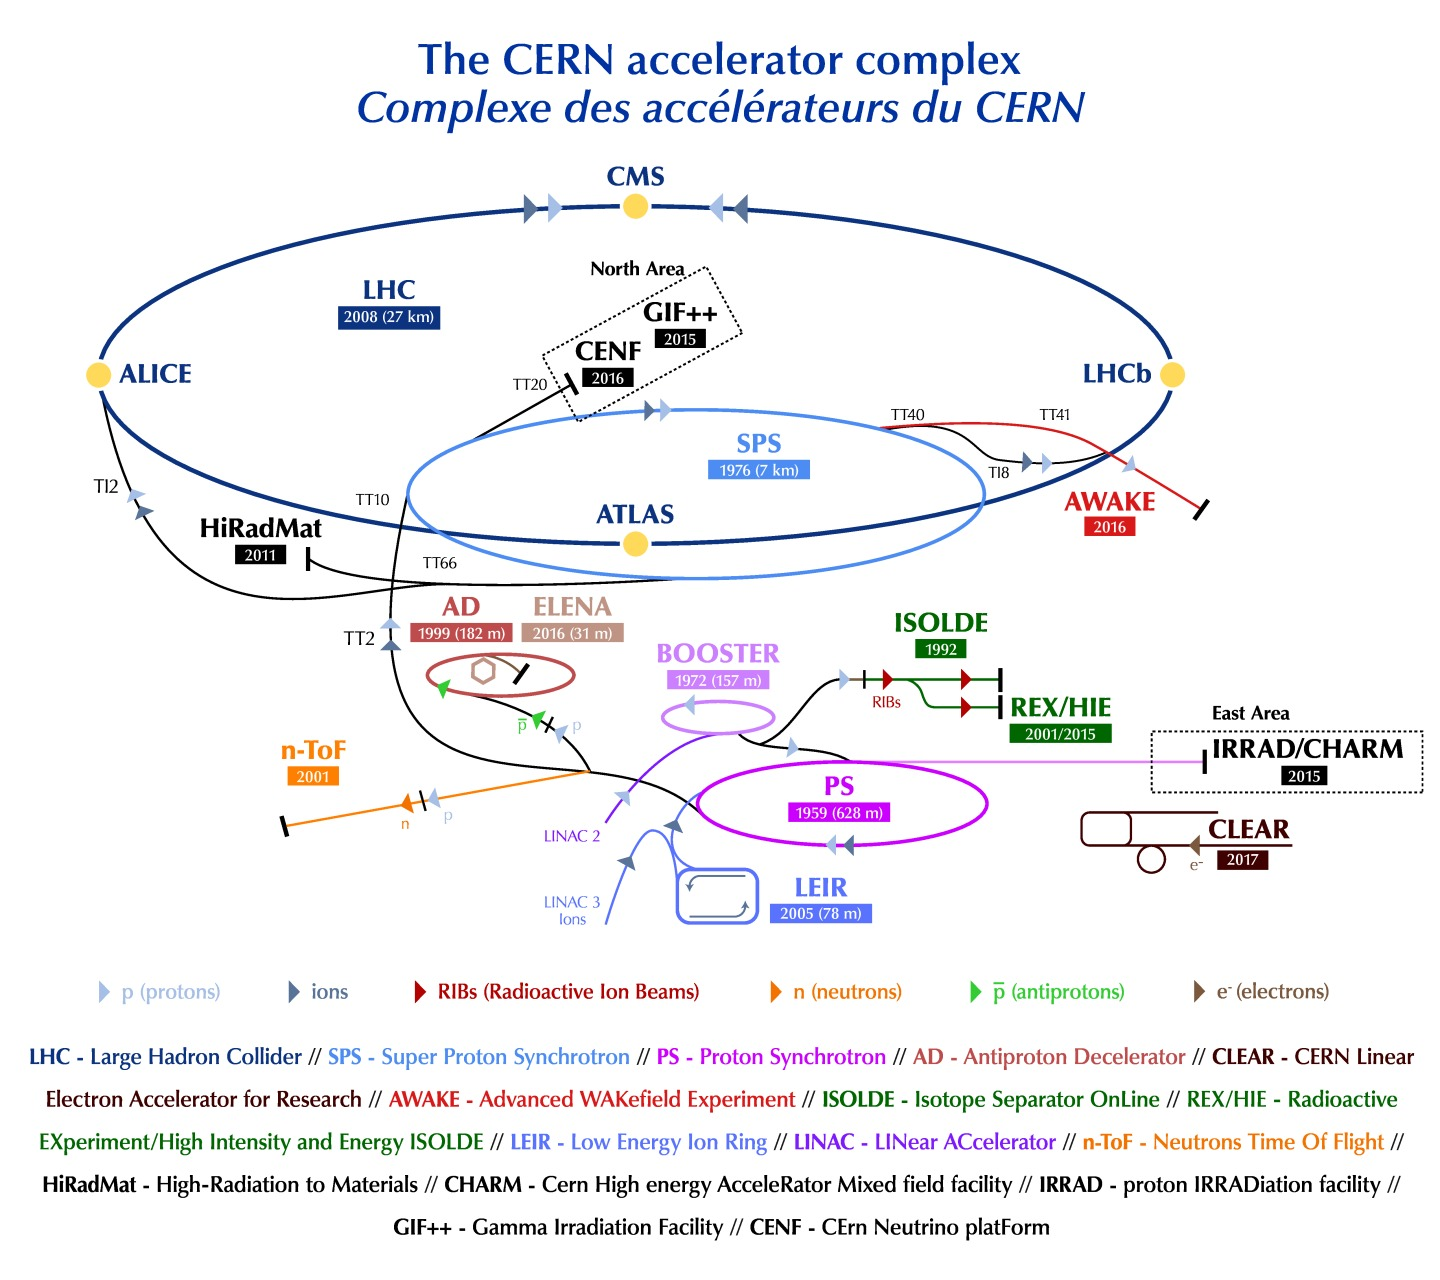
\includegraphics[width=0.9\textwidth]{Figures/Apparatus/cernmachines.jpg}
\caption[The CERN Accelerator Complex]{The CERN Accelerator Complex~\cite{Mobs:2197559}.}
\label{fig:cernaccelerator}
\end{figure}

The acceleration of protons starts by stripping the electrons on hydrogen atoms originally contained in a hydrogen bottle via a duoplasmatron proton source. Next, those protons are injected and accelerated successively by the LINAC-II, Booster, PS and SPS machines. The SPS output is a beam of protons organized in bunches with energy of 450 GeV, which is injected to the two LHC rings (one in clockwise and other in counter-clockwise direction). The two LHC beams are circulated in opposite directions and accelerated until they achieve an energy of around 6.5 TeV. Once the beams are stable, proton bunches with around $10^{11}$ protons each are collided. 

The LHC is a powerful tool that is capable to achieve high energy to probe the behavior of matter and its interactions. It is a circular superconducting accelerator and collider with 26.7 km of circumference, which is designed to produce pp collisions at up to 14 TeV of center-of-mass energy ($\sqrt{s}$) by colliding proton bunches every 25 nanoseconds in four interaction points (IPs) along the ring. There are experiments located at each of these points: ATLAS (A Toroidal LHC ApparatuS) and CMS (Compact Muon Solenoid) are general-purpose experiments that concentrate on measurements of SM processes and BSM physics searches at the TeV scale, the LHCb (LHC-beauty) experiment focuses on B-hadron physics, and ALICE (A Large Ion Collider Experiment) studies heavy-ion collisions phenomena (e.g. quark-gluon plasma). 

A key parameter to describe the collider operation is the instantaneous luminosity ($\mathcal{L}$), which depends on the beam properties as described in equation~\ref{eq:luminosity} and listed in Table~\ref{tab:lumiparameters}. The LHC operation was originally designed to achieve an instantaneous luminosity of around $\mathrm{10^{34}}$ $\mathrm{cm^{-2}~s^{-1}}$. High luminosities are important because they increase the production rate of interesting physics process, and thus our potential and sensitivity for physics discoveries. However, high luminosities imply the increase of the number of pp interactions per bunch crossing or pile-up (UP), which poses challenges to the experiments for reconstruction and radiation harness.
\begin{equation}
\label{eq:luminosity}
\mathcal{L}=\frac{ N_{b}^{2}~n_{b}~f~\gamma}{4\pi\epsilon\beta\sqrt{1 + (\frac{\theta_{c} \sigma_{z}} {2\sigma^{*}} )^{2} } }    
\end{equation}

The expected number of produced events of a particular process during the LHC collisions (without taking into account the detector acceptance) is predicted as $\mathrm{N=\sigma\cdot~L}$, where $\sigma$ is the theoretical production cross section ($\sigma$), and L is the integrated luminosity (L) defined as the integral of the instantaneous luminosity over the LHC operation time. The units of integrated luminosity are the inverse barn (b$^{-1})$, where $\mathrm{1~b^{-1} = 10^{24}~cm^{-2}}$.

\begin{table}[htb]
\centering
\caption[Parameters used in the calculation of the instantaneous luminosity at the Large Hadron Collider proton-proton collisions]{\label{tab:lumiparameters} Parameters used in the calculation of the instantaneous luminosity at the Large Hadron Collider proton-proton collisions~\cite{Bruning:782076}.}
\begin{tabularx}{\textwidth}{XX}
\hline
LHC design experimental parameters                      & Design or nominal values     \\
\hline
$f$, revolution frequency                               & 11.245 kHz        \\[0pt]
$n_{b}$, number of proton bunches per beam              & 2808              \\[0pt]
$N_{b}$, number of proton per bunch                     & 1.15 x $10^{11}$  \\[0pt]
$\beta$, optical beta function at the IP                & 55 cm             \\[0pt]
$\sigma_{Z}$,  RMS bunch length                         & 7.55 cm           \\[0pt]
$\sigma_{*}$,  transverse RMS beam size                 & 16.7 $\mu$m       \\[0pt]
$\gamma$, relativistic gamma factor                     & 7461              \\[0pt]
$\epsilon$, normalized transverse beam emittance        & 3.75 $\mu$m rad   \\[0pt]
$\theta_{c}$, crossing angle at the IP                  & 285  $\mu$rad     \\[0pt]
\hline
\end{tabularx}
\end{table}

The baseline plan of the LHC at past, present and future operations is presented in Figure~\ref{fig:lhcschedule}. The LHC particle beams were circulated for the first time in September 2008 but days later a failure of an electrical connection produced led to severe damage to the superconducting magnets, their connections and the vacuum pipe. After investigating the problem and over a year of repairing, the LHC beams were circulated back again in November 2009, and the first run of the LHC (Run-I) started at the beginning of 2010.
\begin{figure}[htp!]
\centering
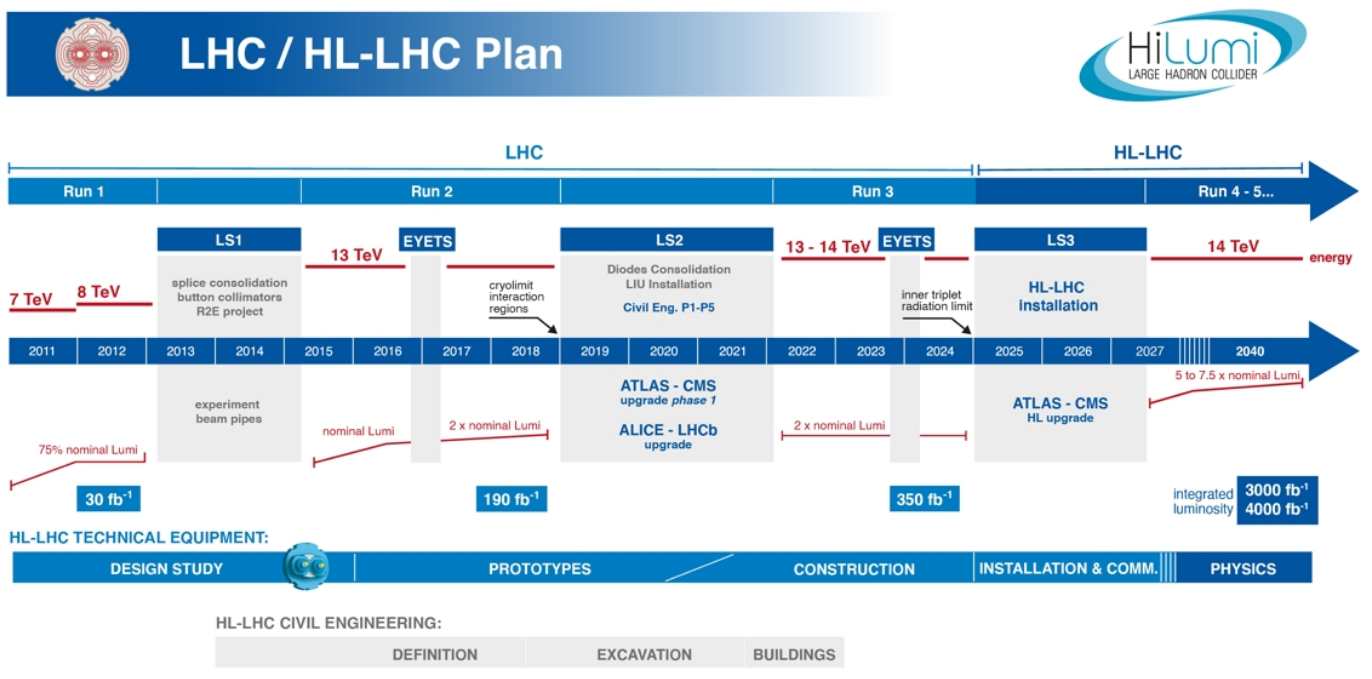
\includegraphics[width=1.0\textwidth]{Figures/Apparatus/lhcschedule.png}
\caption[The Large Hadron Hadron Collider schedule starting from Run-1 operations (2011) to the next decades and beyond.]{The Large Hadron Collider schedule starting from Run-1 operations (2011) to the next decades and beyond. In red, it is presented the expected proton-proton collision center-of-mass energy and the instantaneous luminosity.}
\label{fig:lhcschedule}
\end{figure}

%The LHC Run-1
In the LHC Run-1 (2010-2012), pp collision data was collected at $\sqrt{s}=$ 7 and 8 TeV with bunches crossing every 50 nanoseconds. The collected Run-1 dataset was analyzed for the discovery of the Higgs boson. Then, during the first long shutdown (LS1), 2013-2014, the LHC superconducting magnets were trained for the operation with 6.5 TeV proton beams, thus pp collisions at 13 TeV of center-of-mass energy. Moreover, detector upgrades took place. For instance, the CMS experiment performed the upgrade of its Level-1 trigger (hardware and architecture), in preparation for the Run-2 conditions.

%The LHC Run-2
The Run-2 operation of the LHC took place from 2015-2018, with 13 TeV pp collisions. The LHC reached a record instantaneous luminosity of $\mathrm{2.1~x~10^{34}}$ $\mathrm{cm^{-2}~s^{-1}}$, corresponding to an average of $55$ PU interactions. In CMS, the measured Run-2 average of PU interactions was around 34 as presented in Figure~\ref{fig:cmspileuprun2} A). The total integrated luminosity delivered by the LHC during the Run-2 operations was around 164 $\mathrm{fb^{-1}}$, as presented versus time in Figure~\ref{fig:cmspileuprun2} B). 

\begin{figure}[htp!]
\centering
\captionsetup[subfigure]{justification=centering}
\subfloat[]{\centering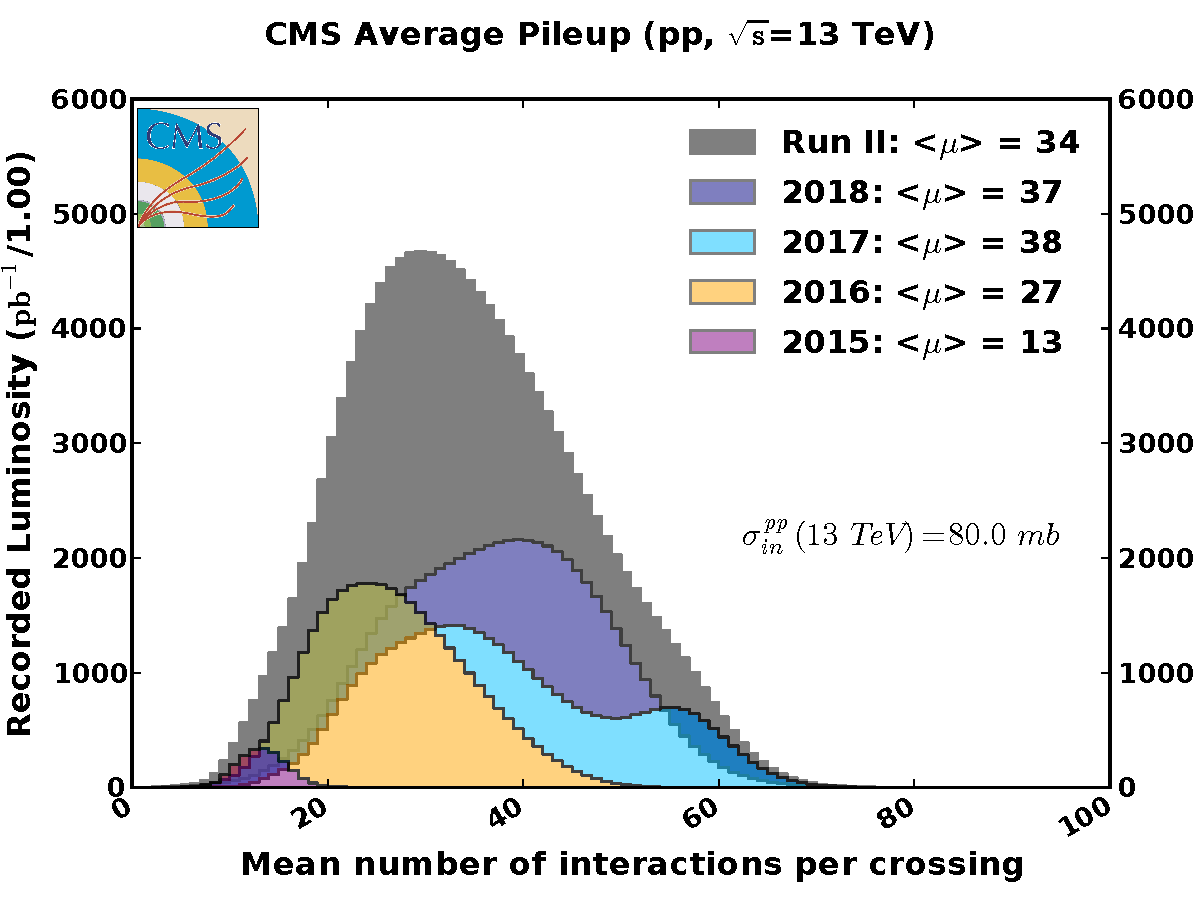
\includegraphics[width=0.45\textwidth]{Figures/Apparatus/pileup_allYears_run2.pdf}}
\subfloat[]{\centering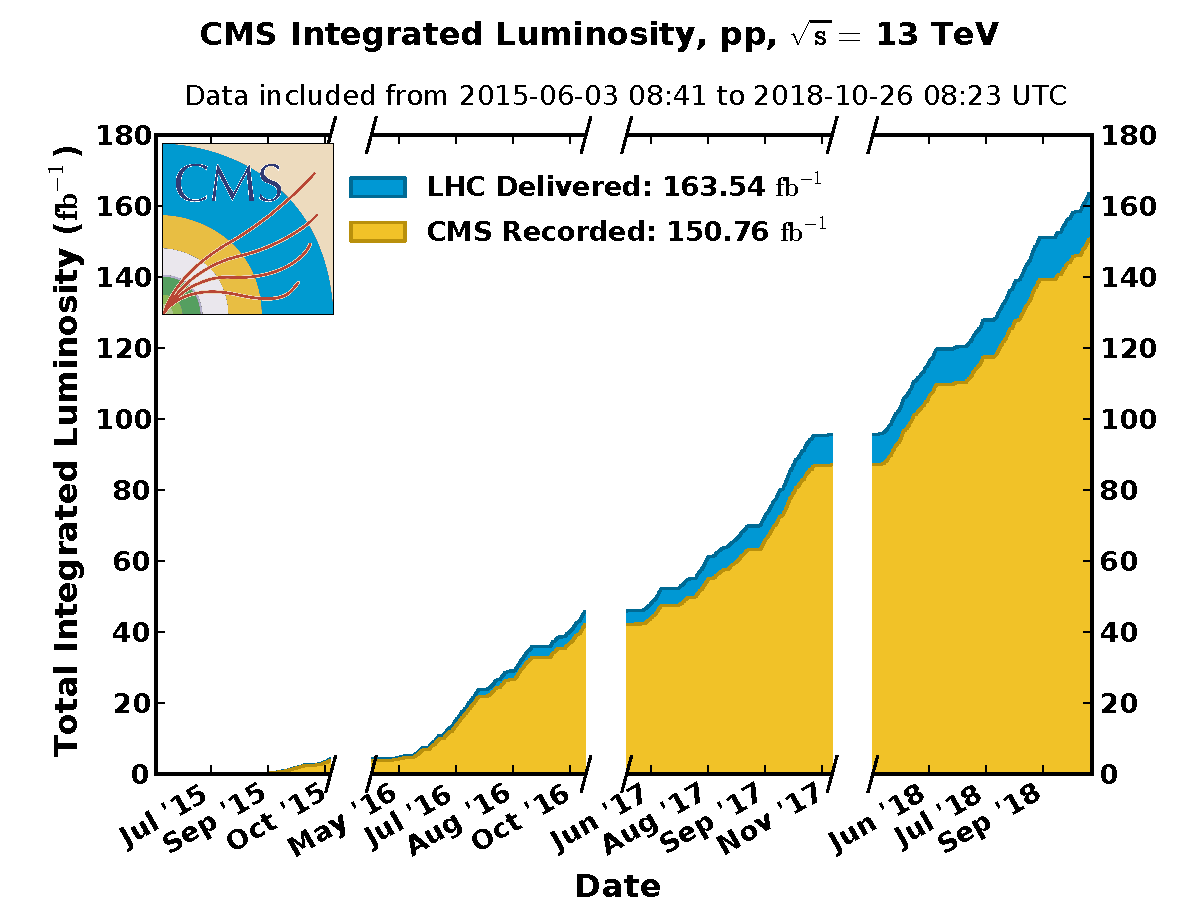
\includegraphics[width=0.45\textwidth]{Figures/Apparatus/int_lumi_allcumulative_pp_run2_cutout.pdf}}
\caption[CMS operation conditions in proton-proton collisions during the LHC Run-2 data-taking]{CMS operation conditions in proton-proton collisions during the LHC Run-2 data-taking. A) Distribution of pile-up average versus recorded luminosity, B) Total integrated luminosity versus time.}
\label{fig:cmspileuprun2}
\end{figure}

%Run-3 and the HL-LHC
At the time of writing this dissertation, the LHC is going under the second long-shutdown (LS2), 2019--2021, in preparation for the Run-3 operations. Due to the current Covid-19 pandemic, the LHC schedule has been delayed. Run-3 is expected to start at the beginning of 2022, and to last until 2024 or 2025. Then, after the third long shutdown (LS3) of 2--3 years, the LHC will operate at its ultimate high luminosity configuration, the HL-LHC. 

The HL-LHC operation period, expected to last for about a decade, is known as the LHC Phase-2. Phase-1 is the current operation until the end of Run-3. The HL-LHC accelerator is expected to produce 14 TeV pp collisions and to reach an instantaneous luminosity of 5--7.5 $\mathrm{x~10^{34}}$ $\mathrm{cm^{-2}~s^{-1}}$, corresponding to 200--300 average PU interactions. The expected dataset corresponds to 3000-4000 $\mathrm{fb^{-1}}$ of integrated luminosity (roughly 20-27 times more data than the one used in this dissertation). Major consolidation and upgrades of the LHC accelerator are ongoing in preparation for the HL-LHC era. The LHC experiments will undergo an important upgrade program to successfully operate in the challenging collision conditions (more in Section~\ref{subsec:cmsupgrades}).

\section{The CMS Experiment}
\subsection{Description}
The Compact Muon Solenoid (CMS) experiment is a general-purpose experimental apparatus located 100 meters underground within a cavern at the LHC Point 5 (P5) in Cessy, France~\cite{CMS:2008xjf}. The CMS detector surrounds the LHC IP with dedicated particle detector layers (or subsystems) to reconstruct the collisions products (electron, muons, photons, charged and neutral hadrons) and study the underlying physics phenomena. This detector has a cylindrical symmetry and is uniquely characterized by a high magnetic field superconducting solenoid. More details on the detector layers are presented by the next subsection.

\begin{figure}[htp!]
\centering
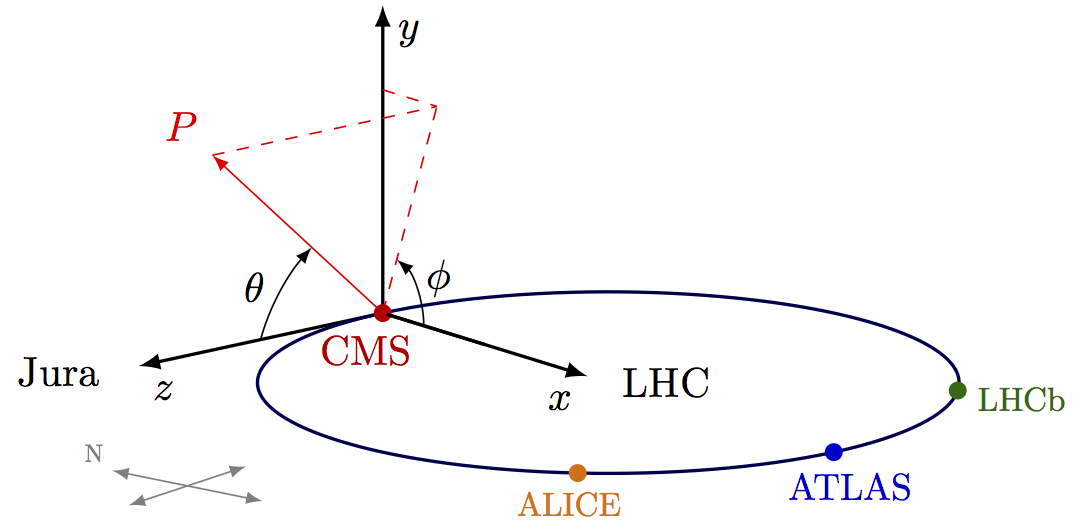
\includegraphics[width=0.95\textwidth]{Figures/Apparatus/cms_coordinate_system.png}
\caption[The CMS conventional coordinate system]{The CMS conventional coordinate system.}
\label{fig:coordinates}
\end{figure}

The conventional coordinate system used by CMS is illustrated in Figure~\ref{fig:coordinates}. The origin is fixed at the interaction point inside the detector. The X-axis points towards the center of the LHC, the Y-axis is perpendicular to the plane defined by the LHC ring, and the Z-axis is parallel to the beam line following the anticlockwise direction. The azimuthal angle $\phi$ is measured with respect to the X-axis over the X-Y plane. The polar angle $\theta$ is defined with respect to the Z-axis over the Y-Z plane.  The
$\theta$ angle is converted to the variable pseudorapidity $\eta$ by the relation $\eta=-\ln{[\tan{(\frac{\theta}{2}) }]}$. The angular distance between two points is measured in units of $\mathrm{\Delta R=\sqrt{ (\Delta\phi)^{2} + (\Delta\eta)^{2} }}$. The transverse component of vectorial properties such as the momentum are defined as the projection of the vector in the X-Y plane (e.g. transverse momentum $\mathrm{p_{T}}$). 

\subsection{Detector Layers}
At the LHC design luminosity, an average of 20 pile-up interactions are expected to occur simultaneously at the interaction point every 25 nanoseconds. Consequently, detectors with large number of channels and good timing resolution are needed to reconstruct and identify the products of the interaction under study with respect to the other interactions in the same bunch crossing. Moreover, the high-particle multiplicity environment ($\sim$1000 charged particles per bunch crossing) produce high radiation levels which can cause detector damage and thus, radiation-hard detectors/electronics are needed.

The CMS detector was designed to conduct a successful physics program involving diverse final states under the aforementioned data-taking constraints by satisfying the following detector requirements~\cite{CMS:2008xjf}:
\begin{itemize}
    \item Muon identification with good reconstructed momentum resolution ($<10\%$ at P$\sim$1 TeV)
    \item High momentum resolution and reconstruction efficiency of charged-particles
    \item Efficient triggering of $\tau$ leptons and b-quark hadronic jets
    \item Good resolution and efficient leptons and photons energy and isolation measurements
    \item Good missing-transverse energy measurement and dijet-mass through a hermetic, granular and angular coverage 
\end{itemize}

\begin{figure}[ht!]
\centering
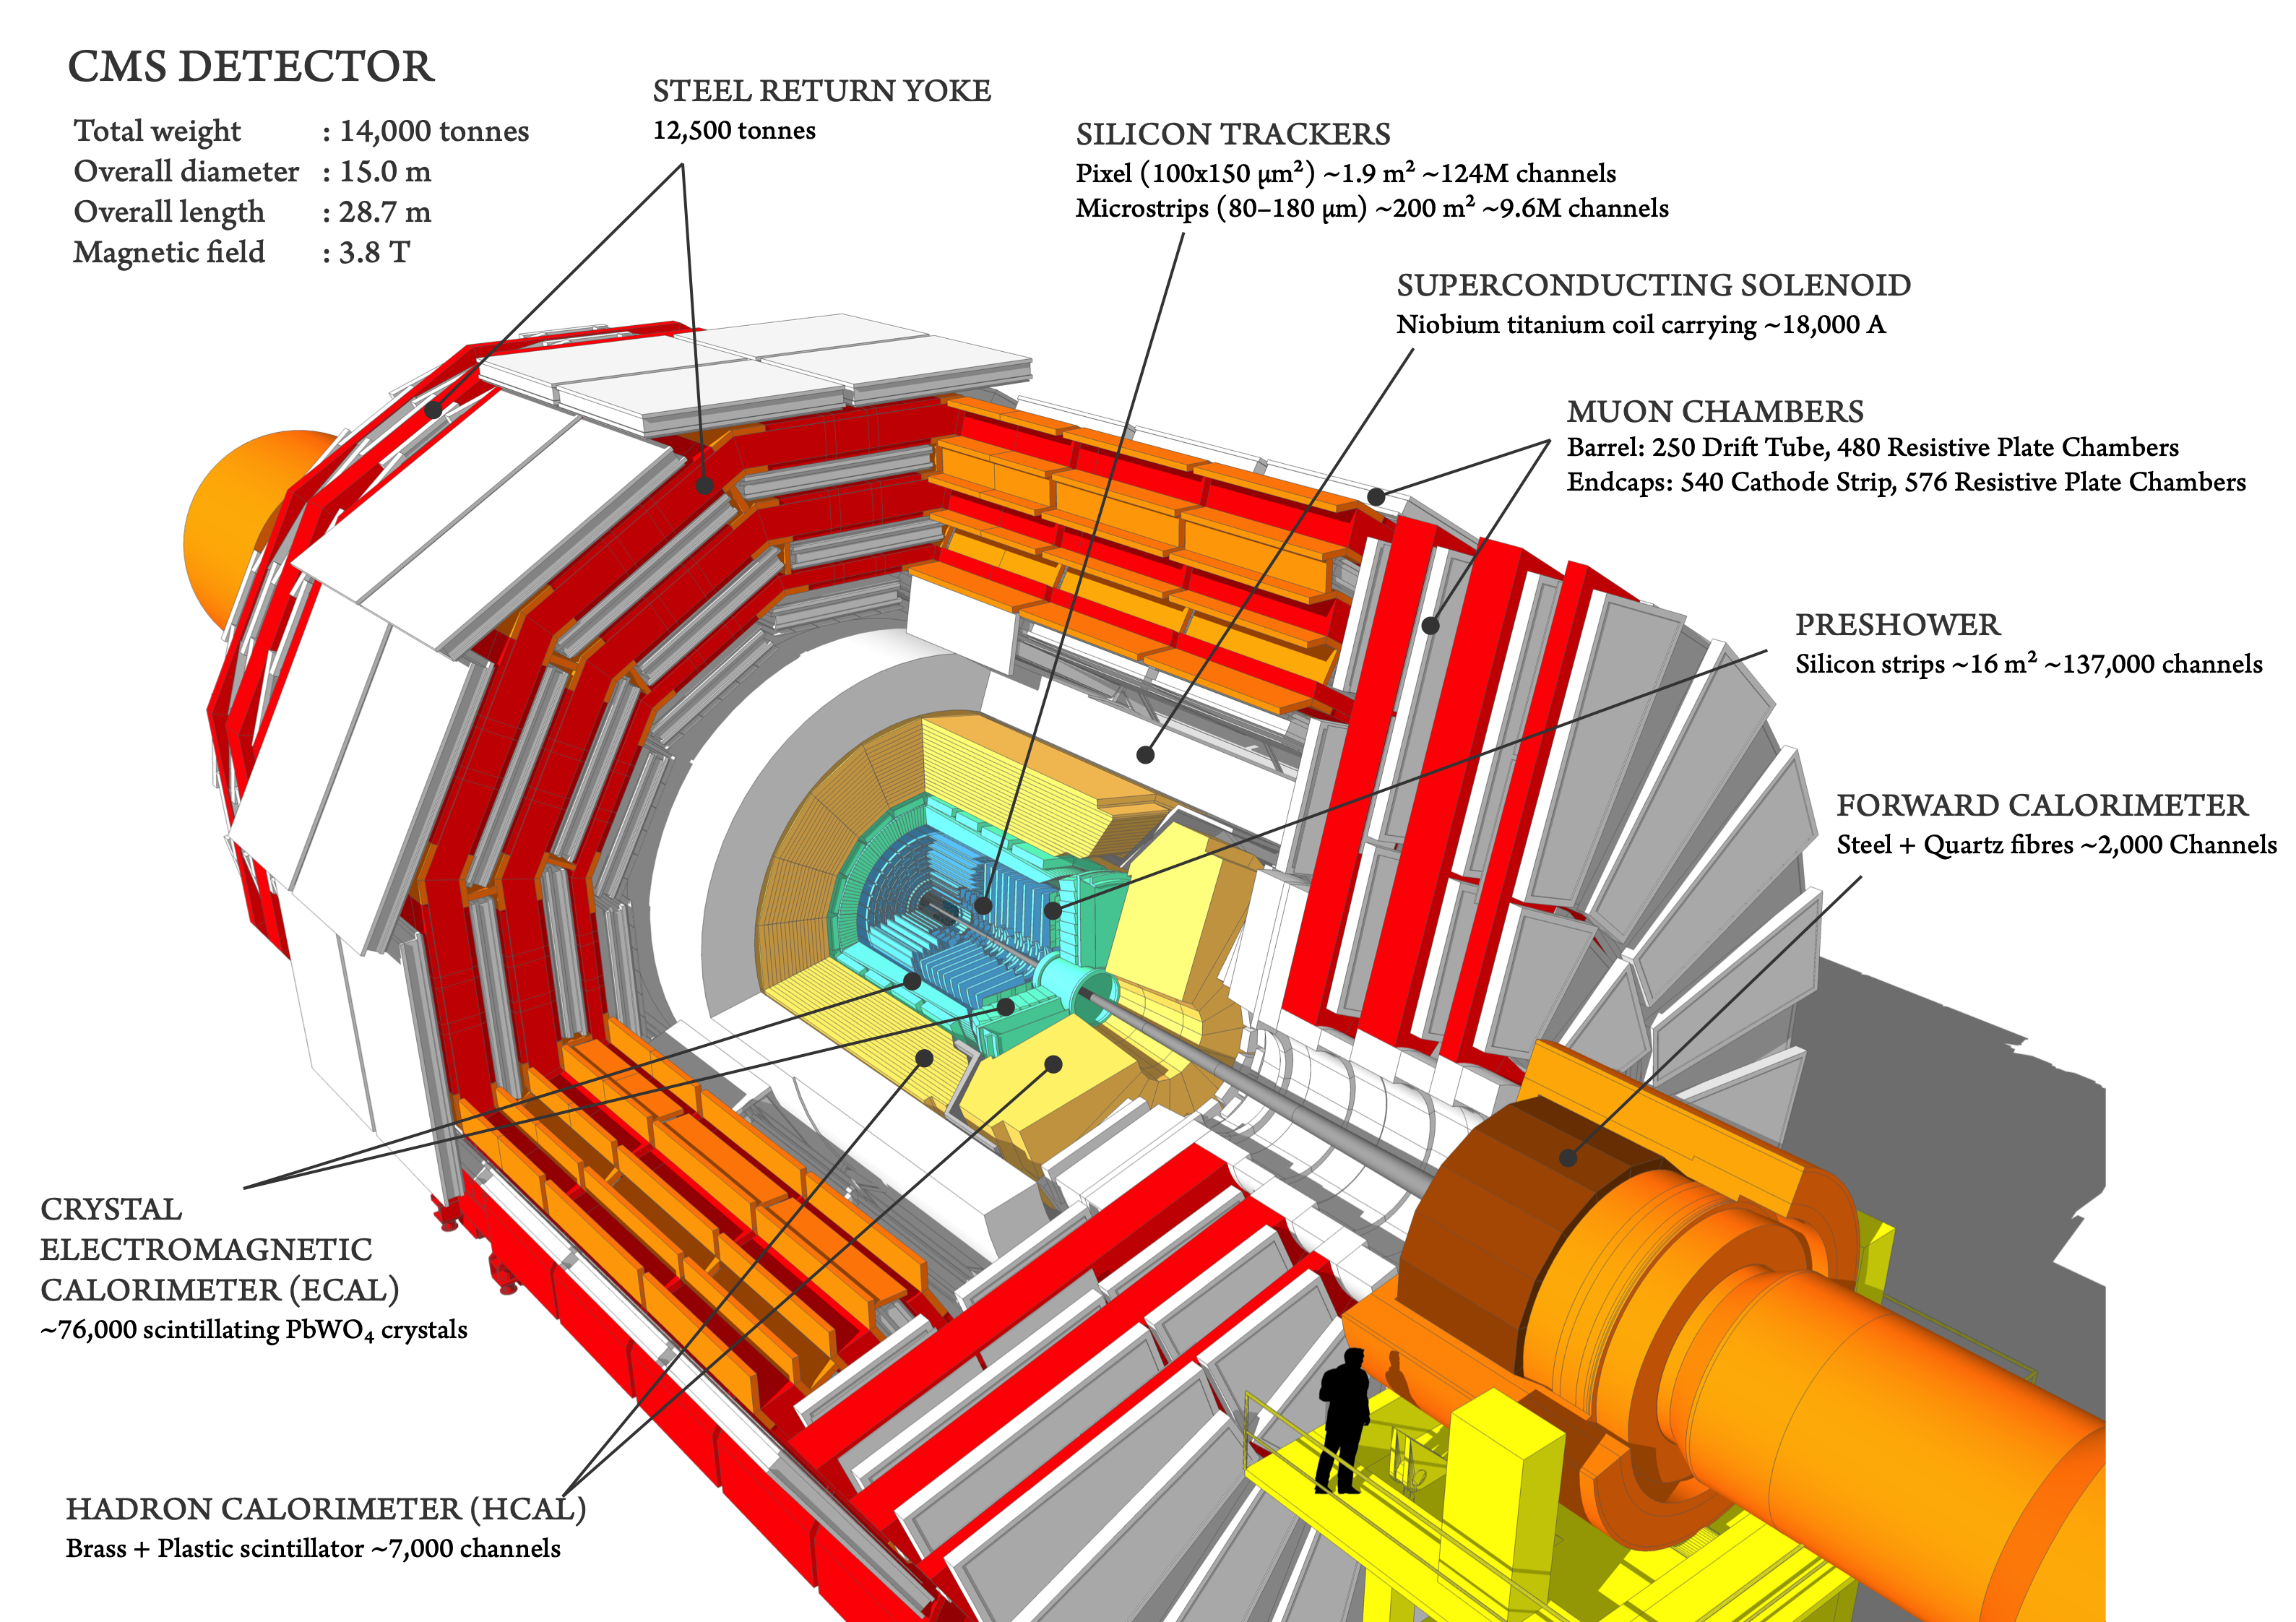
\includegraphics[width=1.0\textwidth]{Figures/Apparatus/cmsdetector.png}
\caption[Three-dimensional view of the subdetectors of the CMS experiment]{Three-dimensional view of the subdetectors of the CMS experiment.}
\label{fig:cmsdetector}
\end{figure}

The CMS detector layout and dimensions are presented in Figure~\ref{fig:cmsdetector}. A tracker, an electromagnetic and a hadron calorimeter are contained within the superconducting solenoid volume. The first detector layer is a full silicon-based inner tracking system composed of pixels and strip trackers, which information is processed to detect the interaction of charged particles and measure their trajectory and momentum. The energy of electromagnetic particles (photon and electrons) is measured from their energy deposits in a hermetic and homogeneous electromagnetic calorimeter layer made of lead tungstate (PbWO$_{4}$) crystals. Then, a hadronic calorimeter layer with a wide and hermetic coverage measures the energy of deposits from charged and neutral hadrons (e.g. pions). Then, the solenoid is surrounded by the muon system, which embedded in a steel flux-return yoke~\cite{CMS:2008xjf}.

\subsubsection{Inner tracking systems}
%motivation, purpose and capacity
The purpose of the inner tracking system is to provide an efficient and precise measurement of the trajectories of charged particles ($|
\eta|<2.5$), and to reconstruct the points of interactions of protons, referred to as vertices. This system has a primary importance to reconstruct the points of decay of B hadrons away from the beam line, or secondary vertices, which provide the main input to the jet flavor identification. Furthermore, it brings information for high-level triggers. The detector design has a high granularity, fast response, radiation hardness and as minimum material as possible (to reduce the impact on the momentum resolution from multiple scattering) to operate successfully under high collision rates, high particle flux and radiation levels. 

\begin{figure}[ht!]
\centering
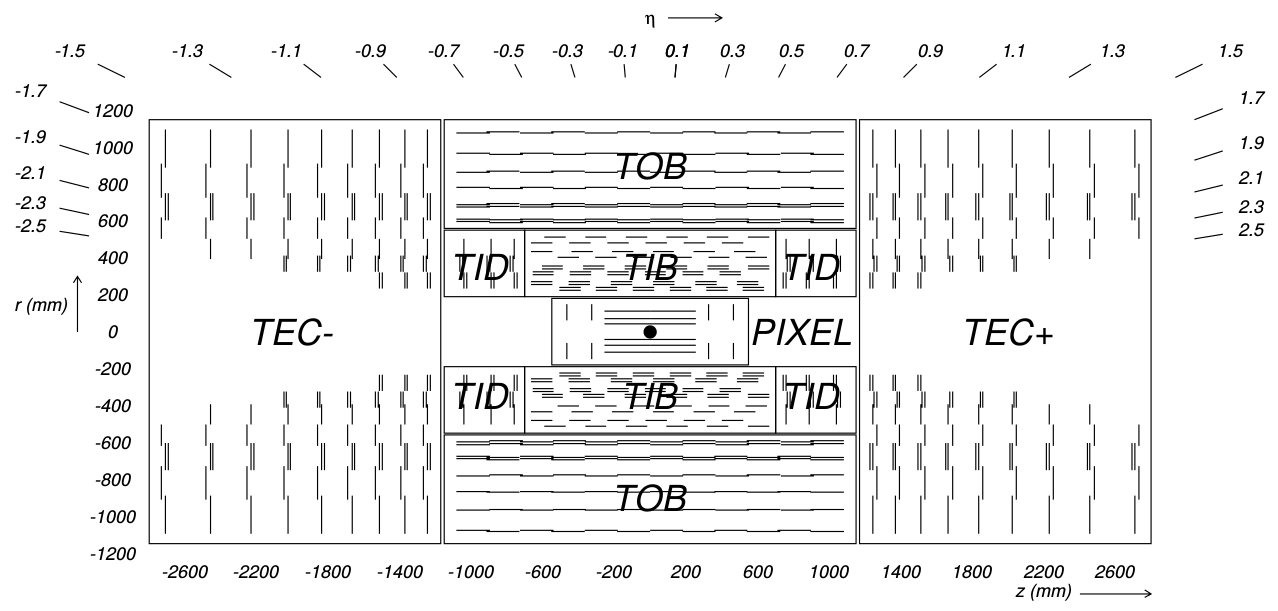
\includegraphics[width=0.9\textwidth]{Figures/Apparatus/cmstrackingsystem.png}
\caption[Layout of the CMS tracking system in the longitudinal direction]{Layout of the CMS tracking system in the longitudinal direction~\cite{CMS:2008xjf}. Note: This layout illustrates the Pixel detector before its upgrade.}
\label{fig:cmstrackingsystem}
\end{figure}
%layout
The layout of tracking system modules is illustrated in Figure~\ref{fig:cmstrackingsystem}. The Pixel tracking detector is the innermost part of the tracking system and thus the closest to the IP. The previous Pixel detector, used until 2016 data-taking, comprised of pixel detector modules organized in three cylindrical layers (BPIX) and two forward/backward disks (FPIX), covering an area of about 1 m$^{2}$ and 66 million pixels with hit resolution between 10-20 $\mathrm{\mu m}$. In the outermost tracking system is the Tracker detector. It comprises detector strip sensors with a total of 9.3 million strips covering 198 m$^{2}$ of area. The strips are organized in three subsystems: Tracker Inner Barrel and Disks (TIB/TID), Tracker outer barrel (TOB), and Track Endcap (TEC). The Tracker covers a pseudorapidity region up to $|\eta|=2.5$~\cite{CMS:2008xjf}.

The new or (upgrade) pixel detector was installed during the 2016/2017 shutdown in preparation for the 2017 data-taking, to maintain and improve the tracking performance under high luminosity conditions (up to $\mathrm{2~x~10^{34}}$ $\mathrm{cm^{-2}~s^{-1}}$ and exceeding an average of 50 pile-up interactions). The new detector consists of four cylindrical layers and three disks~\cite{cmspixelupgrade}. A comparison between the original and new pixel detector organization is illustrated in Figure~\ref{fig:cmstrackingsystemphase1}.

\begin{figure}[ht!]
\centering
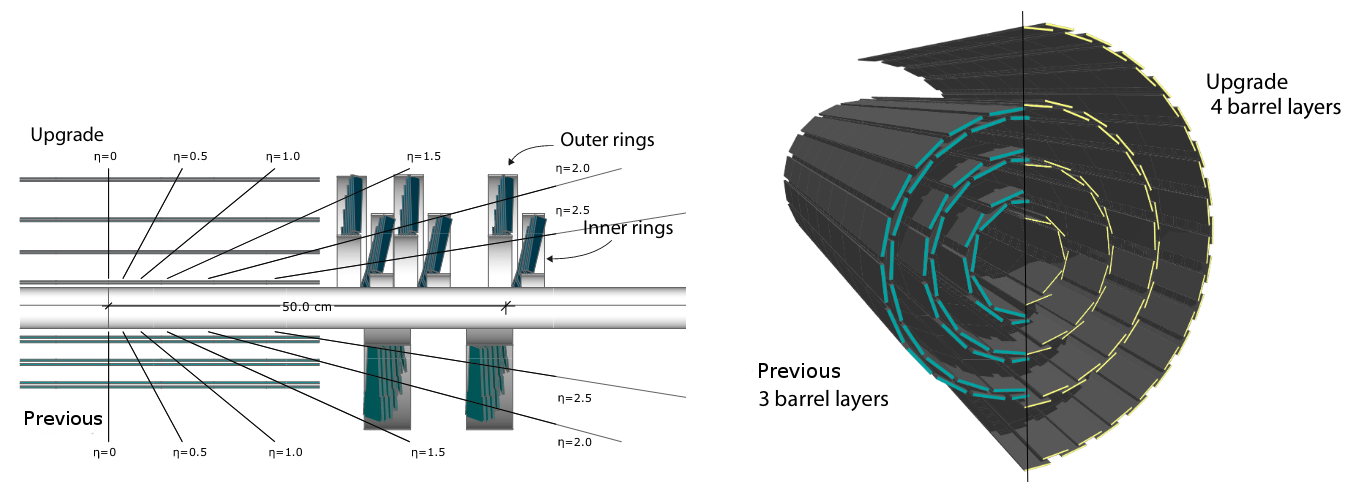
\includegraphics[width=0.9\textwidth]{Figures/Apparatus/cmstrackingsystemphase1.png}
\caption[The CMS pixel detector]{The CMS pixel detector~\cite{cmspixelupgrade}. Left: Half longitudinal section of the pixel detector layout previously (bottom) and after the upgrade (top). Right: Pixel barrel layers geometry previously (left) and after the upgrade (right).}
\label{fig:cmstrackingsystemphase1}
\end{figure}

\subsubsection{Electromagnetic calorimeter}
The electromagnetic calorimeter (ECAL) design was motivated in part by the goal of identifying two photons from the postulated Higgs boson. ECAL is a calorimeter based PbWO$_{4}$ crystals satisfying the requirements to operate under the LHC environment: hermetic, homogeneous, fast, fine granularity and radiation resistant. The radiation length ($X_{0}$) is the average length to reduce the energy of an incident electron by a factor of 1/e. The thickness of ECAL is larger than 25 $X_{0}$. The energy of the electromagnetic showers produced from incident photons/electrons is measured from associated scintillation light as is proportional to the incident particle energy. The scintillation light is collected by avalanche photodiodes (APDs) in the ECAL barrel region (EB, $|\eta|<1.48$), and vacuum phototriodes (VPTs) in the ECAL endcaps (EE, $1.48<|\eta|<3.0$). In addition, a preshower sampling calorimeter (ES) is located in front of the EE section covering $1.65<|\eta|<2.6$, as illustrated in Figure~\ref{fig:cmsecal} A), to help to initiate the electromagnetic showers from incoming photons/electrons, and to identify neutral pion decays into two photons.

The ECAL layout is presented in Figure~\ref{fig:cmsecal} B). A total of 61200 (7234) crystals of front-face cross section of around $\mathrm{22~x~22~mm^{2}}$ ($\mathrm{28.6~x~28.6 mm^{2}}$) and length of 230 (220) mm, are mounted on the EB (EE) region. The EB part is organized in 36 `supermodules', each covering half of the barrel region and divided in four modules. The crystals of the EE region are structured in 2 dees and grouped in units of 5x5 crystals denominated as `supercrystals'~\cite{CMS:2008xjf}.

\begin{figure}[htp!]
\centering
%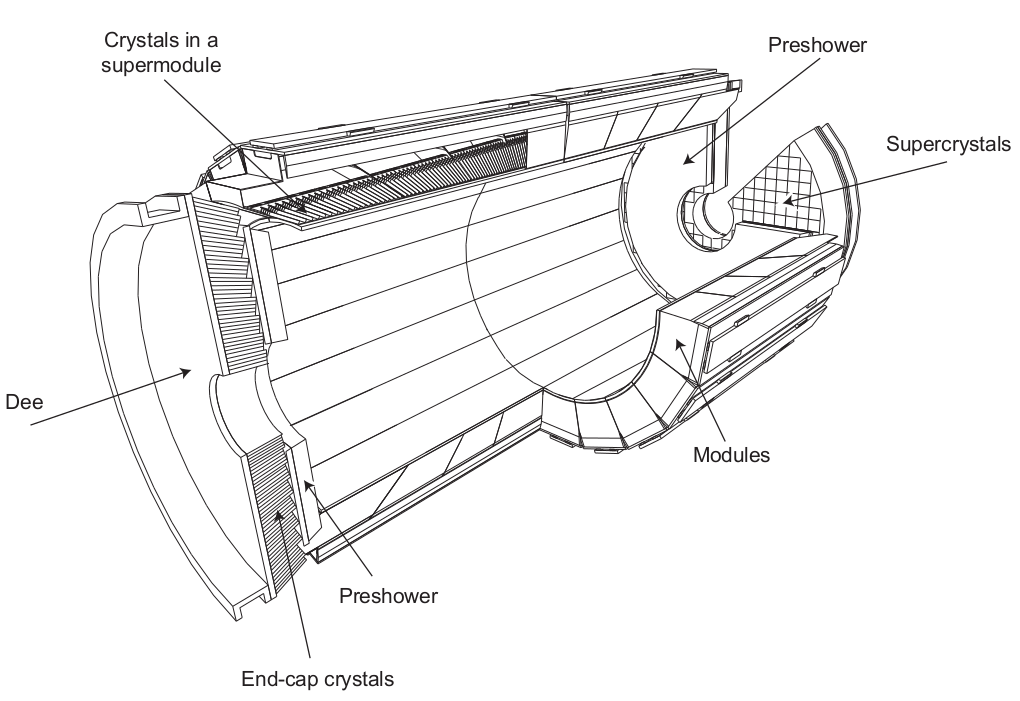
\includegraphics[width=0.9\textwidth]{Figures/Apparatus/cmsecal.png}
\captionsetup[subfigure]{justification=centering}
\subfloat[]{\centering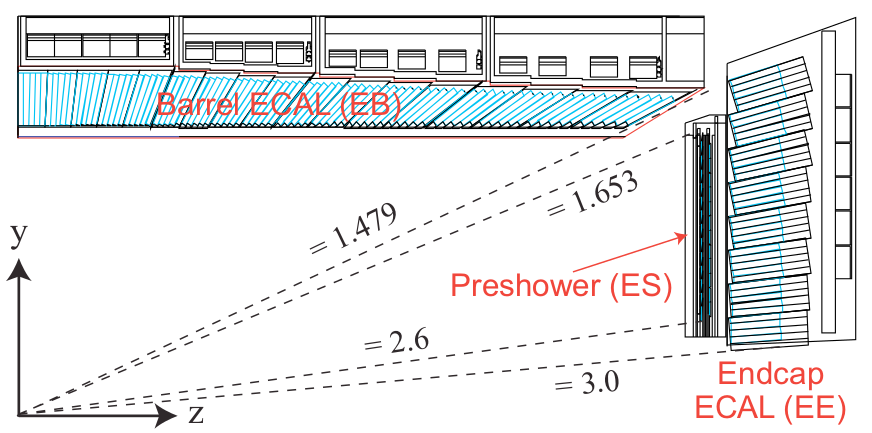
\includegraphics[width=0.43\textwidth]{Figures/Apparatus/cmsecalong.png}}
\subfloat[]{\centering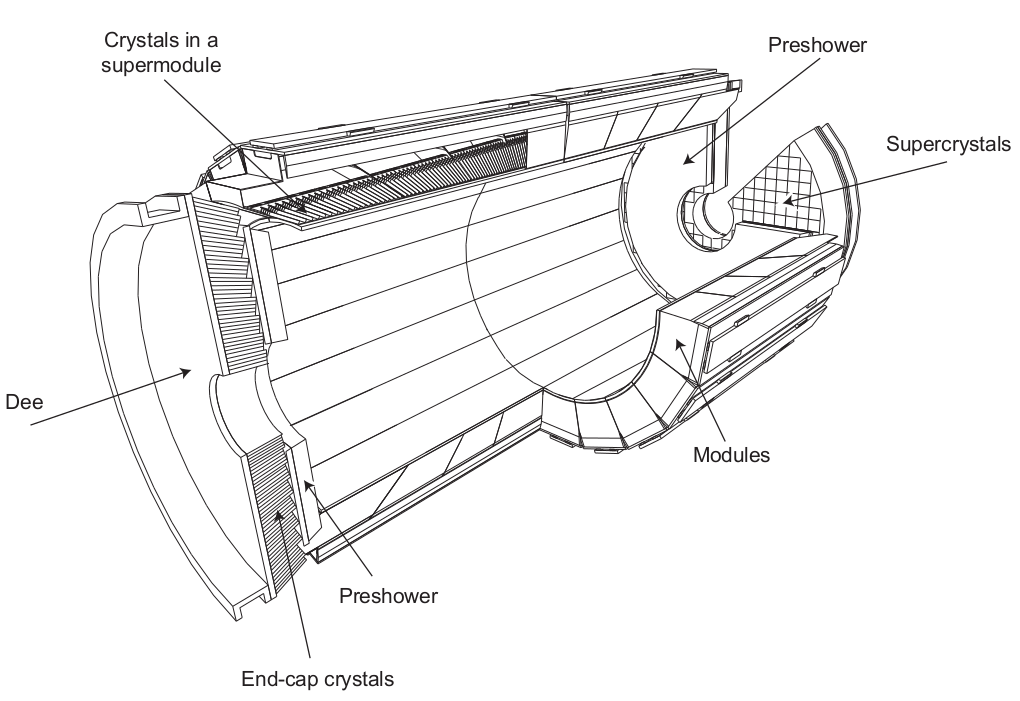
\includegraphics[width=0.43\textwidth]{Figures/Apparatus/cmsecal.png}}
\caption[The CMS electrognetic calorimeter (ECAL)]{The CMS electromagnetic calorimeter (ECAL)~\cite{CMS:2008xjf,CMS:2006myw}. A) Longitudinal section of the geometrical configuration, B) Barrel and endcap configuration layout.}
\label{fig:cmsecal}
\end{figure}

The performance of the ECAL detector was studied through test beam measurements on a barrel supermodule using electron beams of energies between 20 and 250 GeV. The energy resolution ($\mathrm{ \frac{\sigma}{E} }$) can be parametrized as a function of the energy (E) using eq.~\ref{eq:energyresolution}, where S is the stochastic term, N is the noise and C is the constant term. The test beams measured the coefficients to be S=$2.8\%$, N=0.12 and C=$0.30\%$~\cite{CMS:2008xjf}. Then, the energy resolution of the was measured using ${Z\rightarrow e^{+}e^{-}}$ events in the 2010-2011 collision data. The measured resolution of the electrons with $\mathrm{E_{T}}\approx45$ GeV was around 2\% (2-5\%) in $|\eta|<0.8$ (elsewhere)~\cite{cmsecalrun1}. The excellent ECAL calibration and resolution performance were key for the 2012 Higgs boson discovery.
\begin{equation}
\mathrm{\left(\frac{\sigma}{E}\right)^{2} = \left(\frac{S}{\sqrt{E}}\right)^{2} + \left(\frac{N}{E}\right)^{2} + C^{2}}
\label{eq:energyresolution}
\end{equation}

\subsubsection{Hadronic calorimeter}
The hadronic calorimeter (HCAL) is an absorber/scintillator sampling calorimeter surrounding ECAL. It measures the energy of charged and neutral hadrons, which is crucial for the reconstruction of hadronic jets and the missing transverse energy from neutrinos (or exotic particles). Incident hadrons interact with the absorber via nuclear force and generate hadronic showers in the absorber and scintillator. Then, the associated scintillator light is collected by wavelenghth-shifting fibres (WLS) and channeled to photodetectors for readout. The interaction length ($\mathrm{\lambda_{I}}$) of a material is the average distance a hadron travels before an inelastic nuclear interaction. Depending on $\eta$, the HCAL thickness varies within 10-15 $\mathrm{\lambda_{I}}$, and thus a good containment of the hadronic shower~\cite{CMS:2008xjf,CMS:2006myw}. HCAL is divided by four subdetectors: Hadron barrel (HB, $|\eta|<1.4$), Hadron outer (HO), Hadron Endcap (HE, $1.3<|\eta|<3.0$) and Hadron forward (HF, $3.0<|\eta|<5.0$). The layout of the HCAL detector is presented in Figure~\ref{fig:cmshcal}.

\begin{figure}[ht!]
\centering
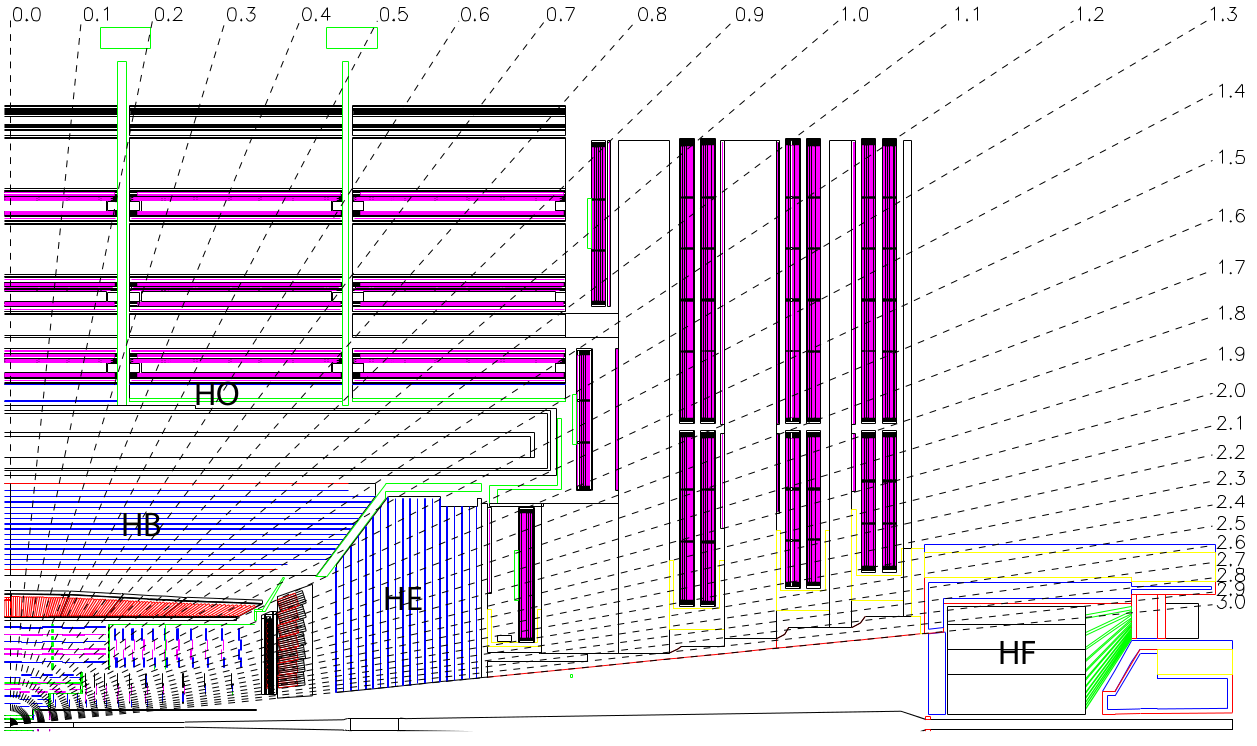
\includegraphics[width=0.8\textwidth]{Figures/Apparatus/cmshcal.png}
\caption[Longitudinal layout of the CMS hadronic calorimeter (HCAL)]{Longitudinal layout of the CMS hadronic calorimeter (HCAL)~\cite{CMS:2008xjf}.}
\label{fig:cmshcal}
\end{figure}

The HB and HE are brass/plastic scintillator tiles sampling calorimeters located inside the solenoid. In the HB and HE sections, there are a total of 2304 readout `towers' formed from the scintillator tiles with a  segmentation of $\mathrm{(\Delta\eta,\Delta\phi)=(0.087,0.087)}$ and $\mathrm{(\Delta\eta,\Delta\phi)=(0.17,0.17)}$, respectively. The HCAL photodetectors are multichannel hybrid photodiodes (HPDs). HO and HF subdetectors are located outside the solenoid. The HO subdetector provides additional layers of scintillator to sample the energy of hadron showers leaking from the rear of the calorimeters, improving the $\mathrm{E_{T}}$ resolution. The HF calorimeters, located at around 11 meters from the interaction point, consist of steel absorber and quartz-fiber layers. Signals come from the Cerenkov light emitted from the quartz fibers, which is collected by photomultipliers (PMTs). The HF materials were chosen in order to contain hadronic showers from energetic forward jets in the intense radiation levels in the forward region~\cite{CMS:2008xjf,CMS:2006myw}.

%Maybe here write about the HCAL+ECAL performance in jet energy or MET resolution
\subsubsection{Superconducting solenoid}
The CMS superconducting solenoid (or magnet) plays a key role in bending the trajectories of charged particles to perform a precise measurement of their transverse momentum using the tracking and muon systems.  An artistic illustration of the CMS magnet is presented in Figure~\ref{fig:cmsmagnet}. It is design to reach a 4 T magnetic field and 2.6 GJ of stored magnetic energy within a cylindrical region with 6 m of diameter and 12.5 m of length. The magnet `cold mass' consist of a 4-layer winding of a reinforced NbTi conductor within a cryostat operating at 1.2 K~\cite{CMS:2008xjf,CMS:2006myw}. 

\begin{figure}[htp!]
\centering
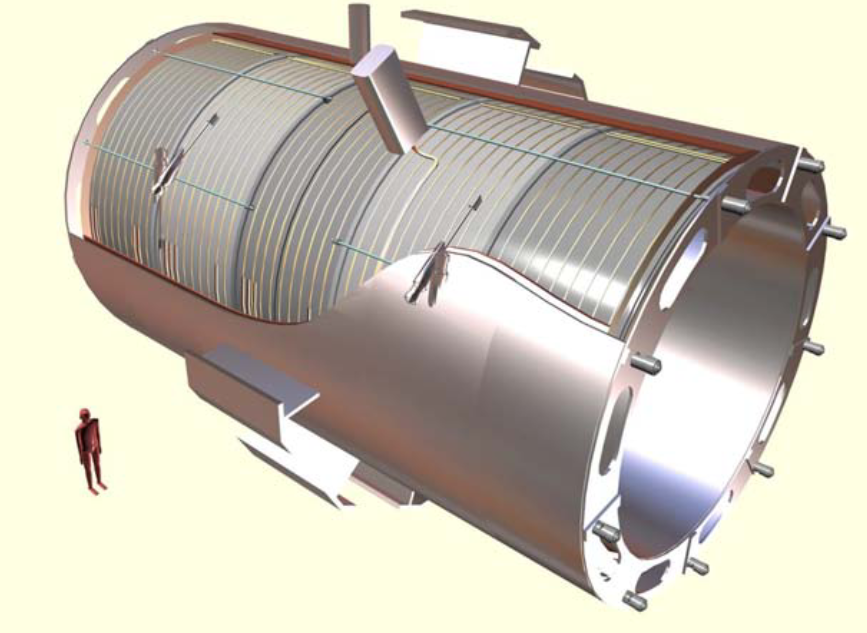
\includegraphics[width=0.8\textwidth]{Figures/Apparatus/cmsmagnet.png}
\caption[Three-dimensional artistic view of the CMS magnet]{Three-dimensional artistic view of the CMS magnet~\cite{CMS:2008xjf}.}
\label{fig:cmsmagnet}
\end{figure}

The magnetic flux is returned through an iron yoke, which comprises 5 wheels (-2,-1,0,1,2) in the barrel region, and two endcaps, as seen in Figure~\ref{fig:cmsdetector}. The iron yoke holds the detectors of the muon system, and it serves as hadron absorber.

\subsubsection{Muon system}
The precise measurement of muons is crucial in the CMS experiment because those particles are produced in many interesting signatures. One example is the Higgs boson decay into a Z boson pair with four muons in the final state ($\mathrm{H\rightarrow ZZ\rightarrow4\mu}$), which was the golden channel in the Higgs boson discovery due to the excellent mass resolution. The muon system is designed for muon identification, precise momentum and charge reconstruction, and triggering over the kinematic range of the LHC. In Figure~\ref{fig:cmsmuonsystem} is illustrated the layout of the CMS muon system and its three types gaseous chambers: Drift tubes (DTs)~\cite{cmsdtscosmicrays}, Cathode strip chambers (CSCs)~\cite{cmscscscosmicrays} and Resistive Plate Chambers(RPCs)~\cite{cmsrpcscosmicrays}. Depending on $\eta$, different detector types are mounted to achieve an efficient detector response in the full region of $|\eta|<2.4$~\cite{CMS:2008xjf,CMS:2006myw}. 

\begin{figure}[ht!]
\centering
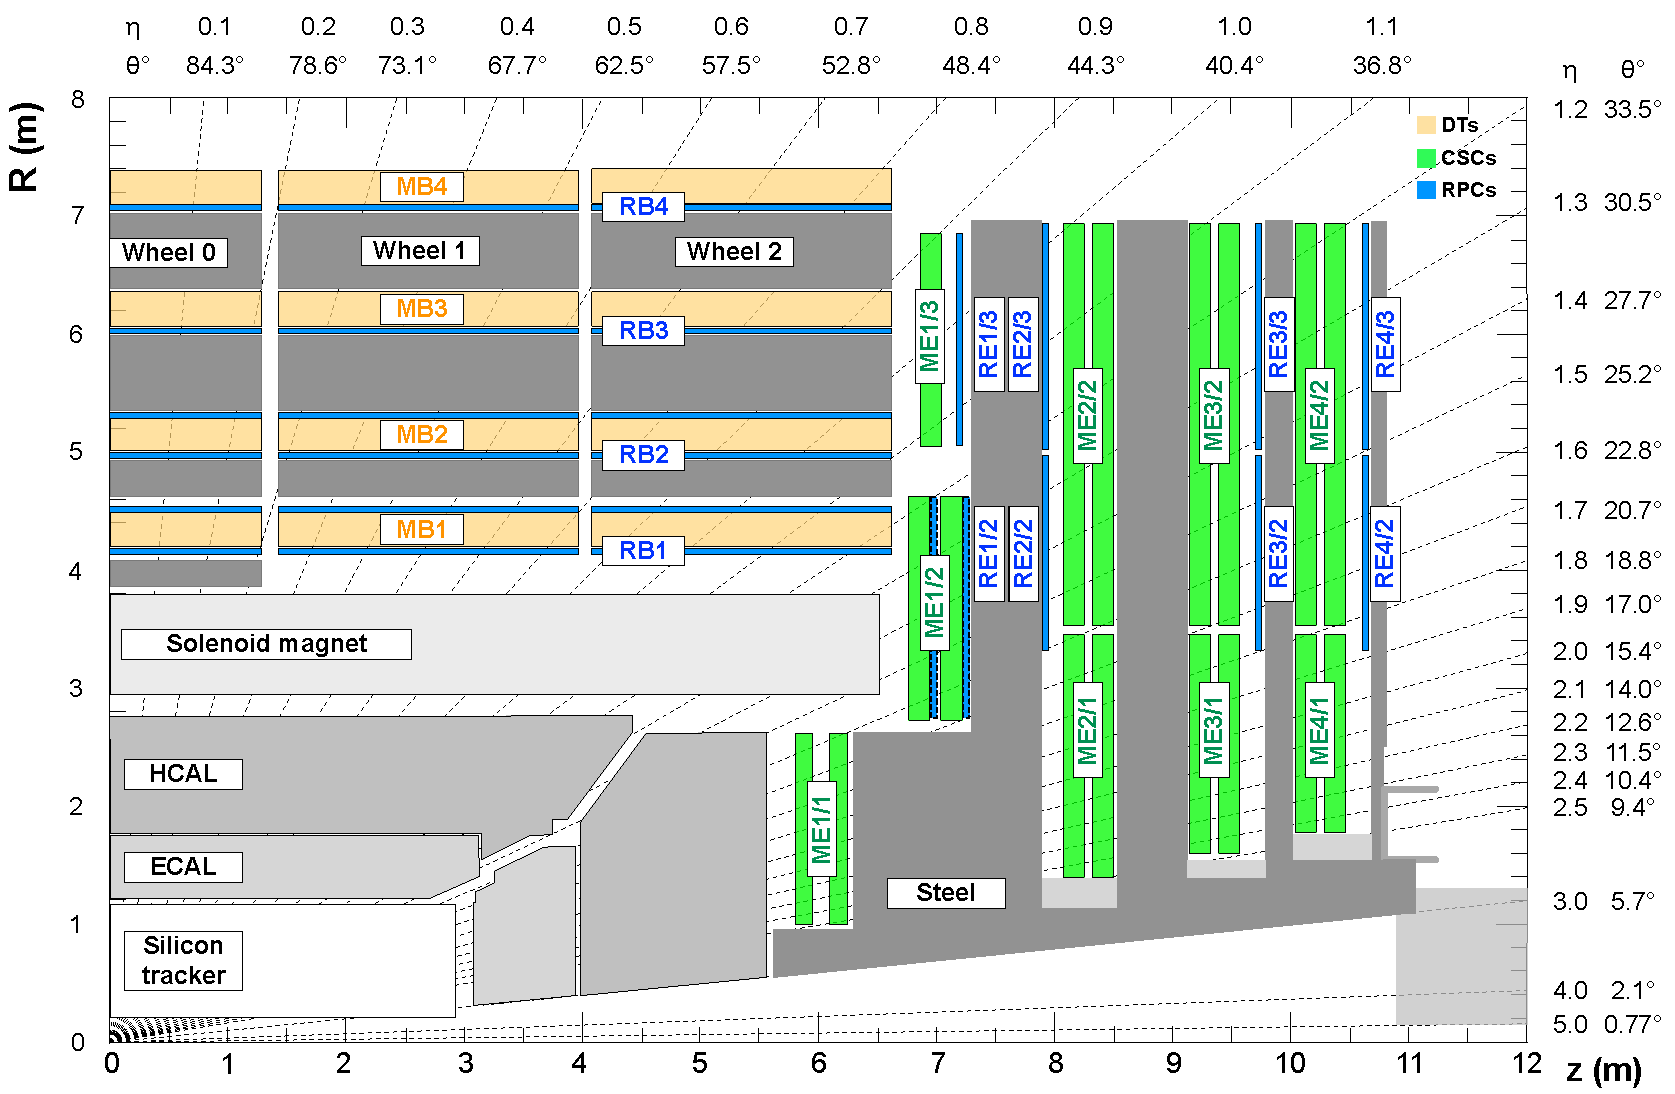
\includegraphics[width=0.9\textwidth]{Figures/Apparatus/cmsmuonsystem.pdf}
\caption[One quadrant of the CMS muon system in the longitudinal direction]{One quadrant of the CMS muon system in the longitudinal direction. Drift tubes (DTs), Cathode strip chambers (CSCs) and Resistive Plate Chambers are presented in orange, green and blue color, respectively.}
\label{fig:cmsmuonsystem}
\end{figure}

In the barrel region, the neutron-induced background is small, the muon rate is low, and the magnetic field is approximately constant. Consequently, a total of 250 DT chambers are used in the $|\eta|<1.2$ region. They are organized in 4 stations (or radial layers) and embedded in the flux-return yoke wheels. In the endcap region, the muon rates and background levels are high, and the magnetic field is not uniform. Therefore, CSCs are used in the $0.9<|\eta|<2.4$ region due to their fast timing, fine segmentation and radiation hardness. A total of 468 CSCs are positioned in the two endcaps. RPCs are characterized by a fast response, good time resolution, but have lower space resolution than CSCs and DTs chambers. A set of RPCs is added in both barrel and endcap regions covering $|\eta|<1.6$, to identify the correct bunch crossing, increase muon hit redundancy to reduce background, and resolve ambiguities from multiple hits in the same chamber~\cite{CMS:2008xjf,CMS:2006myw}. 

\subsection{Event Reconstruction}

A global description of the collision event, where all stable particles are identified, can be achieved by the correlating and combining the detector information associated to their interaction with the different subdetectors (illustrated in Figure~\ref{fig:cmspfslice}). This type of approach is denominated as Particle-Flow (PF) reconstruction, and first was used by the ALEP experiment at the LEP $\mathrm{e^{+}e^{-}}$ collider~\cite{alephpf}. The CMS design properties (e.g. fine-granularity of the detectors) enable the use of the PF reconstruction. Since the first implementation of it for physics analysis in 2009 and triggering in 2010, all physics analyses use PF reconstruction. 

\begin{figure}[ht!]
\centering
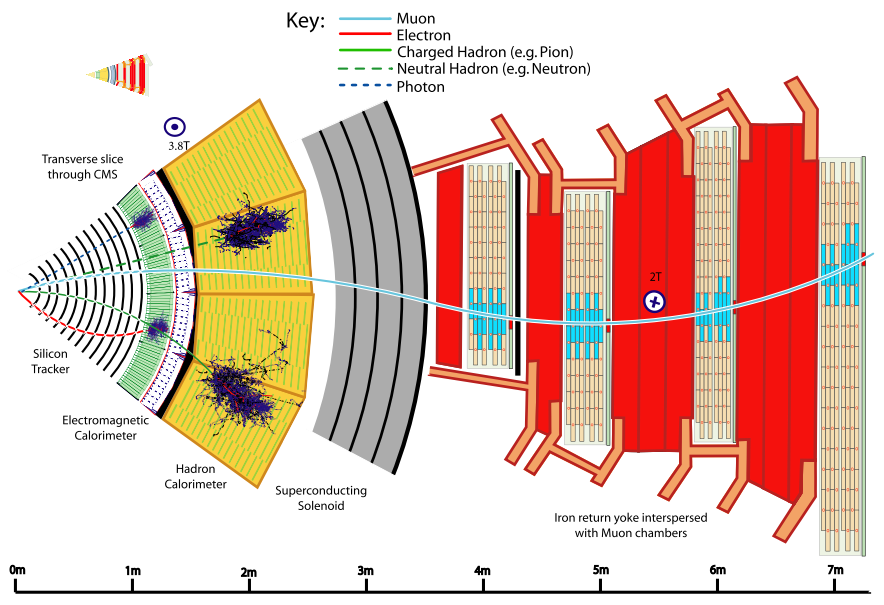
\includegraphics[width=0.95\textwidth]{Figures/Apparatus/cmspfslice.png}
\caption[A transverse slice of the CMS detector representing the interaction of stable particles]{A transverse slice of the CMS detector representing the interaction of stable particles (electron, muon, photon, charged and neutral hadrons) with each of the subsystems.}
\label{fig:cmspfslice}
\end{figure}

The basic PF elements are tracks and calorimeter clusters. Then, they are used for PF identification and reconstruction to produce PF objects/candidates associated to muons, electrons, photons, charged and neutral hadrons. The PF candidates are used after for building more complex physics objects such as hadronic jets, tau leptons, and missing transverse momentum. The PF candidates are the objects used for physics analysis. In what follows it is summarized the CMS methods use to reconstruct all event objects in the context of the PF algorithm. More detailed information is found in Ref.~\cite{cmspfalgo}.

\subsubsection{Tracks and calorimeter clusters}
Experimentalists use track-finder algorithms to find a set of detector hits/stubs compatible with a charged particle track. Then, a fit is performed to obtain the track properties (origin, momentum, direction, etc.). The trajectories of charged particles crossing the CMS inner tracking system (inner track) are reconstructed from hits using an iterative tracking method. In this approach, a combinatorial track finder based on Kalman Filtering (KL) is applied in ten successive iterations. Each iteration has a dedicated seeding and type of track target. The hits associated with built tracks are masked in the next iteration. The reconstruction efficiency surpasses the one from single iteration methods and keeps misreconstruction rates at similar levels~\cite{cmspfalgo}.

The muon system tracking is performed with high efficiency over the different regions of the detector, and independent of the tracker-based or PF reconstruction. There are three possible types of muons:
\begin{itemize}
    \item Standalone muon: The muon track is reconstructed from the information of the CSC, DT and RPC hits using a pattern recognition algorithm for hit selection and a fit method for getting the track properties
    \item Tracker muon: It is an inner track with $\mathrm{p_{T}>0.5~GeV}$ and $\mathrm{p>2.5~GeV}$, which matches with at least one muon hit when extrapolated to the muon system.
    \item Global muon: Standalone muon tracks are matched to inner tracks. Then, for each match that is found, all associated hits are used to fit a global muon track. 
\end{itemize}
A dedicated clustering algorithm is used to generate clusters from the energy deposits in the calorimeters. The clustering method is performed independently by ECAL, HCAL and preshower detectors. In essence, the clustering is as follows. First, cluster seeds are found based on cells passing a seed threshold and larger energy with respect to their neighbors. These neighbors can be the four cells sharing a side (HCAL) or eight cells sharing corners and sides (ECAL and preshower). Then, topological clusters are formed by adding to the seed cluster more cells with at least a common corner and energy twice the noise level. Lastly, an algorithm based on a Gaussian-mixture model reconstruct the clusters with position and energy from the topological cluster. This clustering method applied at HF because the electromagnetic or hadronic component of a cell can be separated into HF EM cluster and HF HAD cluster, respectively~\cite{cmspfalgo}. 

\subsubsection{Particle-flow identification and reconstruction}

In the PF algorithm, the process starts with an algorithm that links PF elements based on the nearest neighbors obtained with a k-dimensional tree across the $(\eta,\phi)$ plane. The link conditions depend on the PF elements involved. The output is called PF blocks, consisting of PF elements with a direct or indirect (via common elements) links. Then, the next step is to identify and reconstruct the particles in each PF block~\cite{cmspfalgo}. 

%Muons
Muons are the first identified particles in the PF block. The muon identification is performed based on the global-muon and tracker-muon properties. The identification minimizes the muon misidentification of charged hadrons. Isolated global muons are identified by taking into account the characteristics of the surrounding tracks and calorimeter deposits within $\mathrm{\Delta R}=0.3$. Non-isolated global muons are identified using tight-muon requirements, at least three muon station segments, and calorimeter deposits compatible with muons, reducing the muon misidentification of high-$\mathrm{p_{T}}$ hadrons. The momentum of the muon is the one from the inner track if $\mathrm{p_{T}}<200$ GeV. Otherwise, the $\mathrm{p_{T}}$ associated to the track fit minimizing the $\chi^{2}$ is chosen. Once the PF muon candidates are found, their PF elements are masked against further processing~\cite{cmspfalgo}.

%Electrons and isolated photons
Electrons are the second objects that are studied in the PF block. When electrons propagate in the inner tracker materials, they often emit bremsstrahlung photons before reaching ECAL. These photons can also produce $e^{+}e^{-}$ pairs, they can emit more photons, and so on. The PF algorithm combines the track and calorimeter information for identification and reconstruction, collecting the energy of soft and energetic radiated photons. Isolated photon identification and reconstruction are performed in the same step~\cite{cmspfalgo}

The ECAL-based seeding of electrons uses the information of ECAL clusters ($\mathrm{E_{T}>4~GeV}$), to infer the position of the hits associated to well isolated and energetic electrons. The energy is determined by grouping clusters into superclusters within a small $\eta$ window and extended $\phi$ window, compatible with the electron magnetic bending. The performance of this method relies on gathering all emitted photons, and thus, this approach is not efficient for non-isolated electrons in jets or soft-$\mathrm{p_{T}}$ electrons. Therefore, a tracker-based seeding for electrons is performed to complement the ECAL-based seeding. First, all inner tracks passing a dedicated preselection ($\mathrm{p_{T}>2~GeV}$, number of hits and the fit $\chi^{2}$ cuts) are fitted again with a Gaussian-sum filter (GSF). These GSF tracks are more compatible with the electron hypothesis as account for the large energy losses along the trajectory~\cite{cmspfalgo}. 

In the PF block, the electron candidate is seeded from a GSF track linked to an ECAL cluster with no more than three additional track links, whereas a photon candidate is seeded from a ECAL cluster with $\mathrm{E_{T}>10~GeV}$ and without GSF track link. All ECAL clusters linked to the superclusters or the GSF track are associated to the candidates. Tracks linked to these ECAL clusters are associated to the candidate if the track momentum and the energy of the linked HCAL cluster is compatible with the electron hypothesis. The photon energy is obtained from the total energy of the associated ECAL clusters, which is corrected as a function of energy and $\eta$, to account for any misses during the association process. The photon direction is the one of the supercluster. The electron energy is assigned from corrected ECAL energy and GSF track momentum information, while the electron direction is taken from the GSF track~\cite{cmspfalgo}.  

Non-isolated and isolated PF electron candidates must satisfy a threshold on a multivariate score based on dedicated BDTs trained with up to 14 variables. If photons are isolated from tracks and calorimeter clusters, and the HCAL - ECAL ratio is compatible with the electron hypothesis, then they are classified as PF photons. All tracks and ECAL or preshower clusters associated to the PF electrons and isolated photons are excluded from further processing~\cite{cmspfalgo}.

%Hadrons and non-isolated photons
The last candidates classified in the PF block are charged hadrons (e.g. $\pi^{\pm}$ and protons), neutral hadrons (e.g. neutrons), and non-isolated and soft photons (e.g. $\pi^{0}\rightarrow\gamma\gamma$), typically produced in hadronic processes (e.g. jets). Within the tracker acceptance ($|\eta|<2.4$), all isolated ECAL (HCAL) clusters without a track link are identified as photons (neutral hadrons), while charged hadron candidates are identified from the HCAL clusters with track link. However, beyond the tracker acceptance, there is no distinction between charged and neutral hadrons. In this case, ECAL clusters with a HCAL-link are assumed to be hadron candidates, otherwise, if there is no such link, they are classified as photon candidates. Then, photon and hadron energies are calibrated from their raw calorimeter energies. HF EM and HF HAD clusters are classified as HF photons and HF hadrons, respectively~\cite{cmspfalgo}.

\subsubsection{Jet reconstruction and flavor identification}

The quark or gluon hadronization generates a collimated shower of particles, which experimental signature is known as hadronic jet or jet. The jet is reconstructed using physical objects such as calorimeter towers or clusters (Calo jets), PF candidates (PF jets) or simulated/generated particles (Gen/Ref jets). A jet clustering algorithm determines which objects are included in the jet. A good jet algorithm is infrared and collinear safe, i.e. the set of jets should be unchanged by soft gluon emission and collinear splitting. Typically, the jet algorithms iteratively find two objects in the event which are closest based on a defined metric and combines them. Then, the jet 4-vector is obtained from the sum of all constituent particle 4-vectors. 

In the CMS experiment, the most used jet clustering algorithm is the $\mathrm{anti-k_{T}}$~\cite{Cacciari:2008gp,Cacciari:2011ma}. A radius parameter of R = 0.4 (0.8) is used to reconstruct small-cone jets (large-cone) jets, known as AK4 (AK8) jets. The AK4 PF (Calo) jets are typically used requiring $\mathrm{p_{T}>15 (20)~GeV}$, otherwise they are considered unreliable. The reconstruction of a di-jet simulated event is illustrated in Figure~\ref{fig:recojets}, where it is observed the good performance of PF jets with respect to Calo jets. Note that tracks and clusters produced from PU interactions can impact the performance of the jet reconstruction. This is mitigated with the charged-hadron subtraction (CHS) method, which excludes any charged particles pointing towards reconstructed PU vertices from the jet clustering and assigns the jet 4-momenta correction from the impact of neutral PU particles~\cite{cmspfalgo}.

\begin{figure}[ht!]
\centering
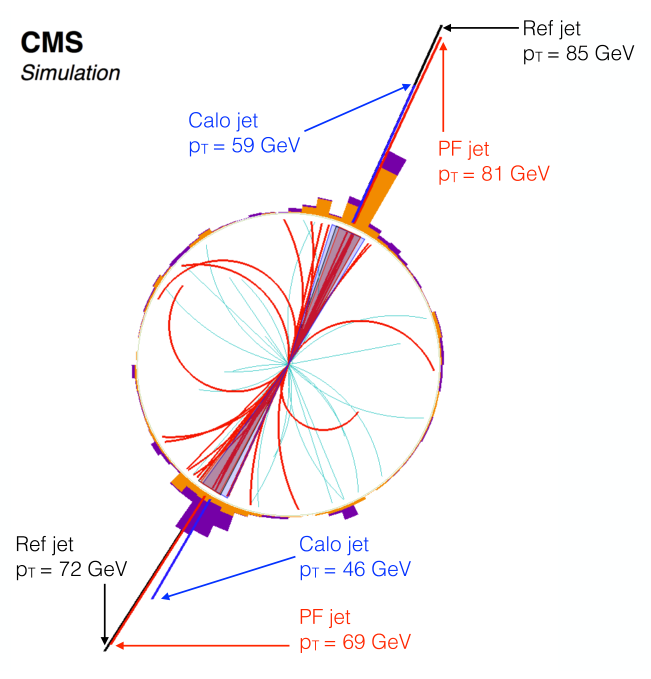
\includegraphics[width=0.6\textwidth]{Figures/Apparatus/dijetreco.png}
\caption[Reconstruction of a di-jet in a simulated event without pile-up]{Reconstruction of a di-jet in a simulated event without pile-up. The jet reconstruction is performed using calorimeter (Calo) jets, PF jets, and generated (Ref) jets. No jet corrections are applied~\cite{cmspfalgo}.}
\label{fig:recojets}
\end{figure}

%JET CORRECTIONS
The reconstructed jets are calibrated to correct their jet energy scale (JES). Jet energy corrections (JEC) as function of $\mathrm{p_{T}}$ and $\eta$ are derived from several dedicated measurements performed using data and simulated events. They address sequentially the impact of pile-up, uniformity of the detector response, and residual data-simulation differences. Furthermore, the jet energy resolution is measured using di-jet and photon+jet events to derive correction for differences between data and simulation. The energy resolution (JER) of central jets is around 15--20\%, 10\% and 5\% for a jet $\mathrm{p_{T} = 30}$ GeV, 100 GeV and 1 TeV, respectively~\cite{CMS:2016lmd}. 
%Jet ID and PU ID
There are jet algorithms developed to reject non-physical jets. Noise jets, originating from calorimeter noise or misreconstruction of electron/muon candidates, are rejected using the PF jet identification criteria, known as PF Jet ID. Moreover, the identification of jets formed from PU particles (PU jets) is performed via the PU ID technique, which permits rejecting those type of jets using a BDT score~\cite{CMS:2017wyc}. 

%Jet b-tagging
Several SM and BSM physics processes have a final state containing heavy-flavor hadronic jets, i.e. jets from b quark (b jets) and c quark hadronization (c jets). Therefore, it is crucial to develop dedicated algorithms for jet flavor assignment or `tagging', to efficiently reconstruct those processes, and reject background associated to light-flavor jets from light-quark and gluon hadronization. Heavy flavor tagging algorithms exploit the physical properties and correlations of the reconstructed jet and its constituents. For instance, one distinctive heavy-flavor jet characteristic is the production of a displaced secondary vertex. As b (c) hadrons (produced during b quark hadronization) have a lifetime of around 1.5 (1) ps, consequently, they have a flight distance a few mm - cm with respect to the primary vertex before decaying into other particles (e.g. charged lepton). The experimental signature is a displaced secondary vertex formed from displaced tracks within the jet. This is illustrated in Figure~\ref{fig:bjet}.

\begin{figure}[htp!]
\centering
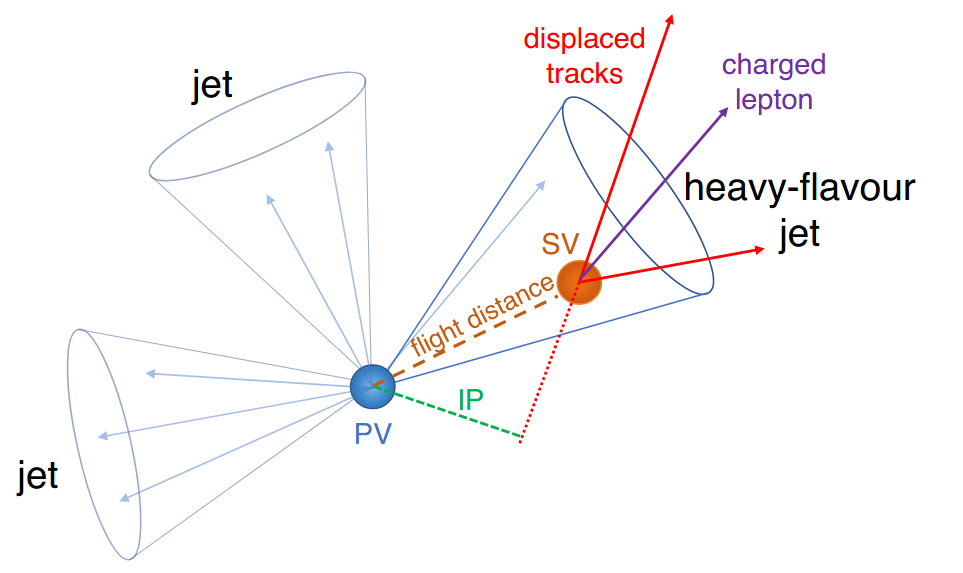
\includegraphics[width=0.5\textwidth]{Figures/Apparatus/bjet.png}
\caption[Heavy-flavour (b quark or c quark) jet kinematic properties]{Heavy-flavor (b quark or c quark) jet kinematic properties~\cite{cmsbtagging13tev}.}
\label{fig:bjet}
\end{figure}

CMS analysts have used heavy-flavor tagging algorithm in data analysis since Run-1~\cite{cmsbtagging8tev}. For Run-2 data analysis, new and more sophisticated algorithms based on deep learning methods have been developed~\cite{cmsbtagging13tev,cmsbtagging13tev2}. The DeepJet algorithm for AK4 jets is the best to date in CMS~\cite{cmsdeepjet}. It is based on a sophisticated deep neural network with a total of 650 inputs from four categories: PF charged candidates, PF neutral candidates, secondary vertex features, and global event variables. The DeepJet multi-output layer is integrated into a multiclassifier which performs b-tagging, c-tagging, and quark/gluon tagging. The performance of this algorithm surpasses significantly the previous algorithms~\cite{cmsbtag1} as illustrated in Figure~\ref{fig:deepjet}. This dissertation uses the DeepJet for b-tagging. 

\begin{figure}[ht!]
\centering
\captionsetup[subfigure]{justification=centering}
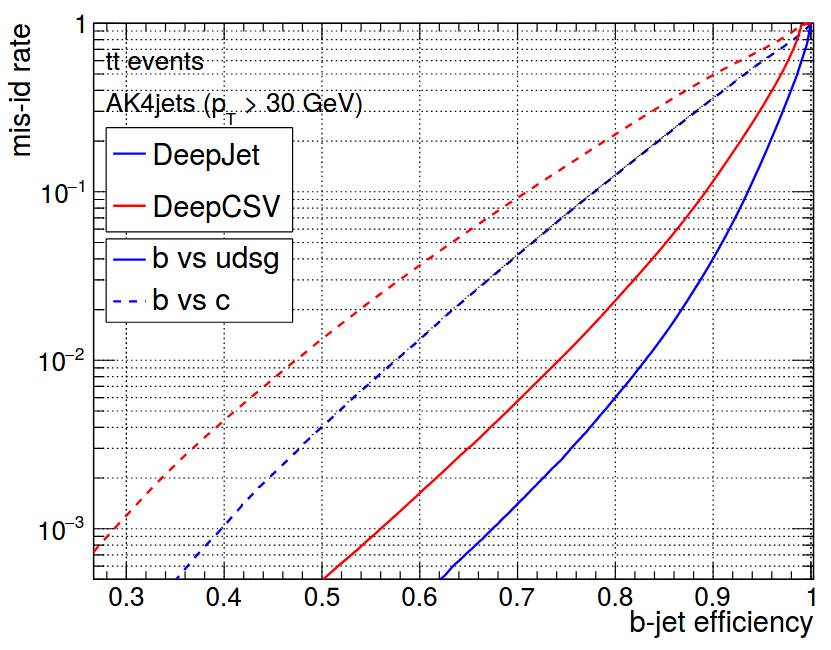
\includegraphics[width=1.0\textwidth]{Figures/Apparatus/deepjet.png}
\caption[Performance of the DeepJet algorithm with respect to the DeepCSV algorithm]{Performance of the DeepJet algorithm with respect to the DeepCSV algorithm in simulated hadronic top quark pair ($\mathrm{t\overline{t}}$) events~\cite{cmsdeepjet}. Mis-id rates vs b-tagging efficiency for jets with $\mathrm{p_{T} > 30 GeV}$.}
\label{fig:deepjet}
\end{figure}

\subsubsection{Tau reconstruction}
The $\tau$ leptons are the most massive charged leptons in Nature (m$_{\tau}\sim1.77$ GeV). The $\tau$-leptonic decays (e.g. $\tau^{-}\rightarrow e^{-} \overline{\nu_{e}}\nu_{\tau}$ ) have a 35.2\% branching fraction. Moreover, $\tau$ leptons are massive enough to have almost all remaining decays involving hadrons (charged hadrons and neutral pions), known as $\tau$-hadronic decays ($\tau_{h}$).

As the two neutrinos escape detection, the $\tau_{l}$ decays are identified through the involved electron or muon candidate. On the other hand, $\tau_{h}$ decays are identified and reconstructed using the Hadron-Plus-Strip (HPS) algorithm since Run-1 data. This method reconstructs the $\tau_{h}$ decay by combining the information from charged hadrons and $\pi^{0}$ candidates. The $\pi^{0}$ candidate is reconstructed by clustering electrons and photons involved in photon conversions within rectangular $\eta~\mathrm{x}~\phi$ regions named `strips'. The main $\tau_{h}$ backgrounds are quark and gluon jets, electrons, and muons candidates. Isolation requirements and a dedicated MVA-based discriminants are used to separate $\tau_{h}$ from jets, electron, and muons. For Run-2 data, the HPS algorithm was modified to have dynamic-size regions to collect more effectively $\pi^{0}$ decay products. Studies on $\tau$ reconstruction using 13 TeV data are presented in Ref.~\cite{cmstau13tev}

\subsubsection{Missing transverse momentum reconstruction}
In a collision event, the presence of particles that do not interact with the detector (e.g. neutrinos) is indirectly inferred from an apparent missing transverse momentum ($\vec{p}_{T}^{miss}$). The precise measurement of $\vec{p}_{T}^{miss}$ is crucial for the study of processes involving neutrinos. A method to determine the uncorrected missing transverse momentum ($\vec{p}_{T}^{miss,raw}$) is defined as the negative sum of the transverse momentum vector of all PF candidates in the event. Some mismeasurement sources are non-linear calorimeter response to hadrons, thresholds on calorimeter energy and track transverse momentum, detector inefficiencies, and pile-up. This is improved by adding the calibrated corrections applied to the PF jets as shown in equation~\ref{eq:met}~\cite{cmspfalgo}. The study of the reconstruction performance of this object at 13 TeV pp collision data is found in Ref.\cite{cmsmet13tev}.
\begin{equation}
\vec{p}_{T}^{miss} = \vec{p}_{T}^{miss,raw} - \sum_{jets} (\vec{p}_{T,jet}^{corr} - \vec{p}_{T,jet}) 
\label{eq:met}
\end{equation}

\subsection{Trigger System}
The LHC proton beams cross at high collision rates (up to 40 MHz). As the detector data payload from a bunch crossing or `event' is around 1 megabyte (MB), the potential data bandwidth is at the order of 100 Terabytes per second (TB/s). There are not currently the resources to store and process this huge amount of information, and consequently, the event rate has to be reduced by a factor of $\approx10^{5}$. At the same time, particle physicists know that there is no need to store all events as most of them are low energy multi-jet events and the interesting events are rare (e.g. the Higgs boson production rate is $\sim1$ Hz).

The trigger is the online filtering system that reduces the event rate to manageable levels and constitutes the first step of the event selection. It only keeps/accepts events with interesting for the CMS physics analyses, reducing the event rate to around 1 kHz. There are two steps (or levels) in which the rate is reduced: (1) Level-1 (L1), and (2) High Level Trigger (HLT)~\cite{CMS:2008xjf,CMS:2006myw}. 

The trigger menu is the set of selection criteria used to cover the physics program with the highest selection efficiency under the trigger rate budget. For instance, a selection criterion (sometimes called trigger path) is to require 2 muons of opposite sign and one with $\mathrm{p_{T}>17}$~GeV and other $\mathrm{p_{T}>10}$~GeV. The L1 and HLT systems have separate menus with typically 300 and 600 trigger paths, respectively. 

Events collected by the trigger then send to the Tier-0 at CERN for tape archival, organization and processing. They are split to one or more primary datasets (PDs) based on the HLT path results, and promptly fully reconstructed for offline physics analysis. Examples of PDs used for this analysis or for associated measurements are: \verb|SingleMuon|, \verb|BTagCSV|, and \verb|JetHT|. 

\subsubsection{The Level-1 Trigger}
The L1 is hardware based subsystem comprising custom designed $\mu$TCA boards using field-programmable gate arrays (FPGAs). This allows a flexible and modular design of algorithms for filtering. The L1 does a fast readout of the event information with a coarse granularity using only the information from calorimeters and muon detectors. However, the L1 system capabilities are constrained by the detector readout electronics. It has up to 4 $\mu$s to make a decision and is limited to a 100 kHz of output rate. The front-end buffers store the full event waiting for the trigger decision from the L1 global trigger~\cite{CMS:2008xjf,CMS:2006myw}.

The current L1 system is not the one used in the LHC Run-1, which was replaced during the year-end technical stop between 2015 and 2016. This upgrade replaced all the hardware, electronic boards, optical links, firmware and software to maintain a high performance for the data-taking condition of the LHC Run-2 and Run-3. The Run-2 performance was excellent and allowed to pursue rich physics program despite the challenges such as increased luminosity, PU, and aging of the subdetectors~\cite{cmsphase1per}. The L1 trigger architecture used during the 2016-2018 operations is illustrated in Figure~\ref{fig:cmsl1triggerarch} and briefly described below: 
\begin{itemize}
    \item Calorimeter (calo) trigger: It combines the inputs from ECAL and HCAL into trigger towers with their corresponding calibrated position and energy at the calo layer 1. Then, hadronic jets, $e/\gamma$ and $\tau$ candidates are formed at the calo layer 2. In each of the objects pile-up subtraction, isolation and calibrations are applied. Then, global quantities such as $\mathrm{E_{T}}$ and MET are computed.
    \item  Muon trigger: It combines the information from the three muon detectors in regional track finders (or Muon Track Finder Layer), where muon tracks are built from the muon segments with $p_{T}$,$\eta$,$\phi$ and quality assignment. There are three independent track finders, each covering specific $\eta$ regions: Barrel Muon Track Finder (BMTF, $|\eta|<0.9$), Overlap Muon Track Finder (OMTF, $0.9<|\eta|<1.2$), and Endcap Muon Track Finder (EMTF, $1.2<|\eta|<2.4$). Then, the Global Muon Trigger ($\mu$GMT) ranks the track finder muons, looks for duplicates and checks for isolation from calo layer 2 trigger towers. Lastly, the best muons are sent to the Global trigger.
    \item Global trigger: It collects all objects from the calo layer 2 and $\mu$GMT. Then, it computes complex properties from those objects and used them in about 500 algorithms called L1 trigger paths. Events satisfying the trigger menu are accepted and sent from the readout buffers to the HLT. 
\end{itemize}

\begin{figure}[ht!]
\centering
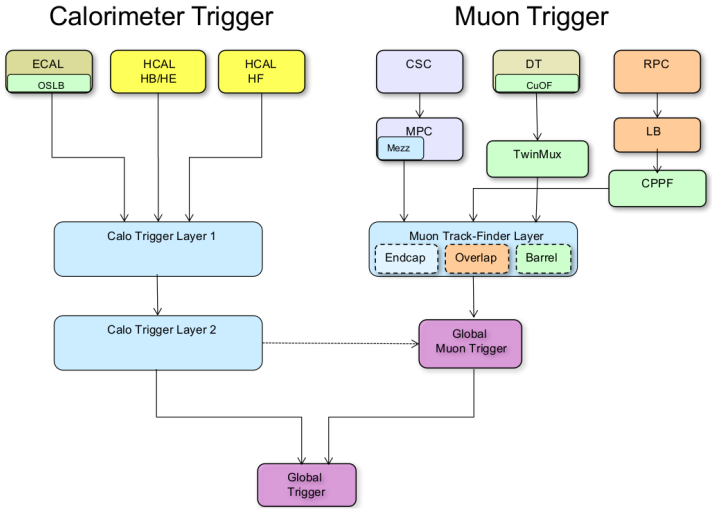
\includegraphics[width=1.0\textwidth]{Figures/Apparatus/cmsl1triggerarchp1.png}
\caption[The CMS Level-1 trigger architecture during the 2016-2018 operations]{The CMS Level-1 trigger architecture during the 2016-2018 operations.}
\label{fig:cmsl1triggerarch}
\end{figure}

\subsubsection{The High Level Trigger}
The HLT is a software based system which algorithms run on a farm of around 26000 commercial CPUs. The HLT algorithms work with higher precision data relative to L1 ones, because it accesses all the event information to perform complex calculations similar to the ones performed during the offline reconstruction. It further reduces the event rate to around 1 kHz. The data bandwidth output is at the order of gigabytes per second (GB/s). The HLT average latency is about 0.3 seconds~\cite{CMS:2008xjf,CMS:2006myw}. 

\subsection{Upgrades in Preparation for the HL-LHC}
\label{subsec:cmsupgrades}
%Write about the HL-LHC
The HL-LHC is the ultimate configuration of the LHC. It is expected to reach an instantaneous luminosity of up to $\mathrm{7.5~x~10^{34}}$ $\mathrm{cm^{-2}~s^{-1}}$. Consequently, over a decade of operation has the potential to delivery an integrated luminosity of 4000~$\mathrm{fb^{-1}}$ to each experiment. To maintain a good data-taking performance and extend the physics selectivity, the CMS experiment will upgrade its subdetectors, electronics, trigger and data acquisition systems. The Phase-2 upgrade will allow for the exploration of a
broad physics program (e.g. scalar sector characterization) to be pursued.     

%write about the phase2 upgrade of detectors
The upgrade of the CMS subdetectors are planned to take place after the Run-3 operations~\cite{cmsphase2proposal}. The preparation is key to achieve an excellent detector response (high granularity, fast readout, radiation hardness) and event object reconstruction under the high particle multiplicity and radiation levels at the HL-LHC~\cite{hllhc}. These upgrades are summarized in the following points:
\begin{itemize}
    \item The inner tracking system will be replaced featuring small size pixel sensors and an Outer Tracker consisting of strip and macro pixel sensors. The extended coverage is up to $|\eta|=3.8$. It will allow reconstructing track candidates for the L1 trigger (L1 tracks) with $|\eta|<2.4$~\cite{cmsphase2tracker}. 
    \item New readout electronics will be installed in the barrel calorimeters. It will provide higher granularity and timing information~\cite{cmsphase2barrelcal}.
    \item The endcap calorimeters will be replaced by a new high granularity calorimeter (HGCAL). This new detector will provide shower separation and identification. It will have both timing and finely segmented energy information~\cite{cmsphase2endcapcal}
    \item The current detectors of the muon system will be kept, but their electronics will be upgraded to provide more accurate information to the L1 trigger. New muon detectors will be installed to improve the coverage (from $|\eta|$ up to 2.4 to 2.8) and redundancy in the forward region. The new detectors are additional improved RPC (iRPC) and gas electron multiplier (GEM) chambers~\cite{cmsphase2muons}. The Phase-2 muon system layout is presented in Figure~\ref{fig:cmsp2upgrade}.
    \item A new timing detector (MTD) will be installed in front of the calorimeters to provide timing measurement of charged tracks with a resolution of about 30-45 picoseconds~\cite{cmsphase2mtd}.
\end{itemize}

%Write about the phase2 upgrade of the trigger the new capabilities
The CMS experiment will keep a trigger with a two-tier strategy at the HL-LHC. The corresponding Phase-2 upgrade of the L1 and HLT systems is currently under design and testing. The first studies of the Phase-2 L1 system capabilities are presented and summarized in the corresponding technical design report (L1TDR)~\cite{cmsphase2l1tdr}, whereas the HLT TDR is under preparation.

\begin{figure}[ht!]
\centering
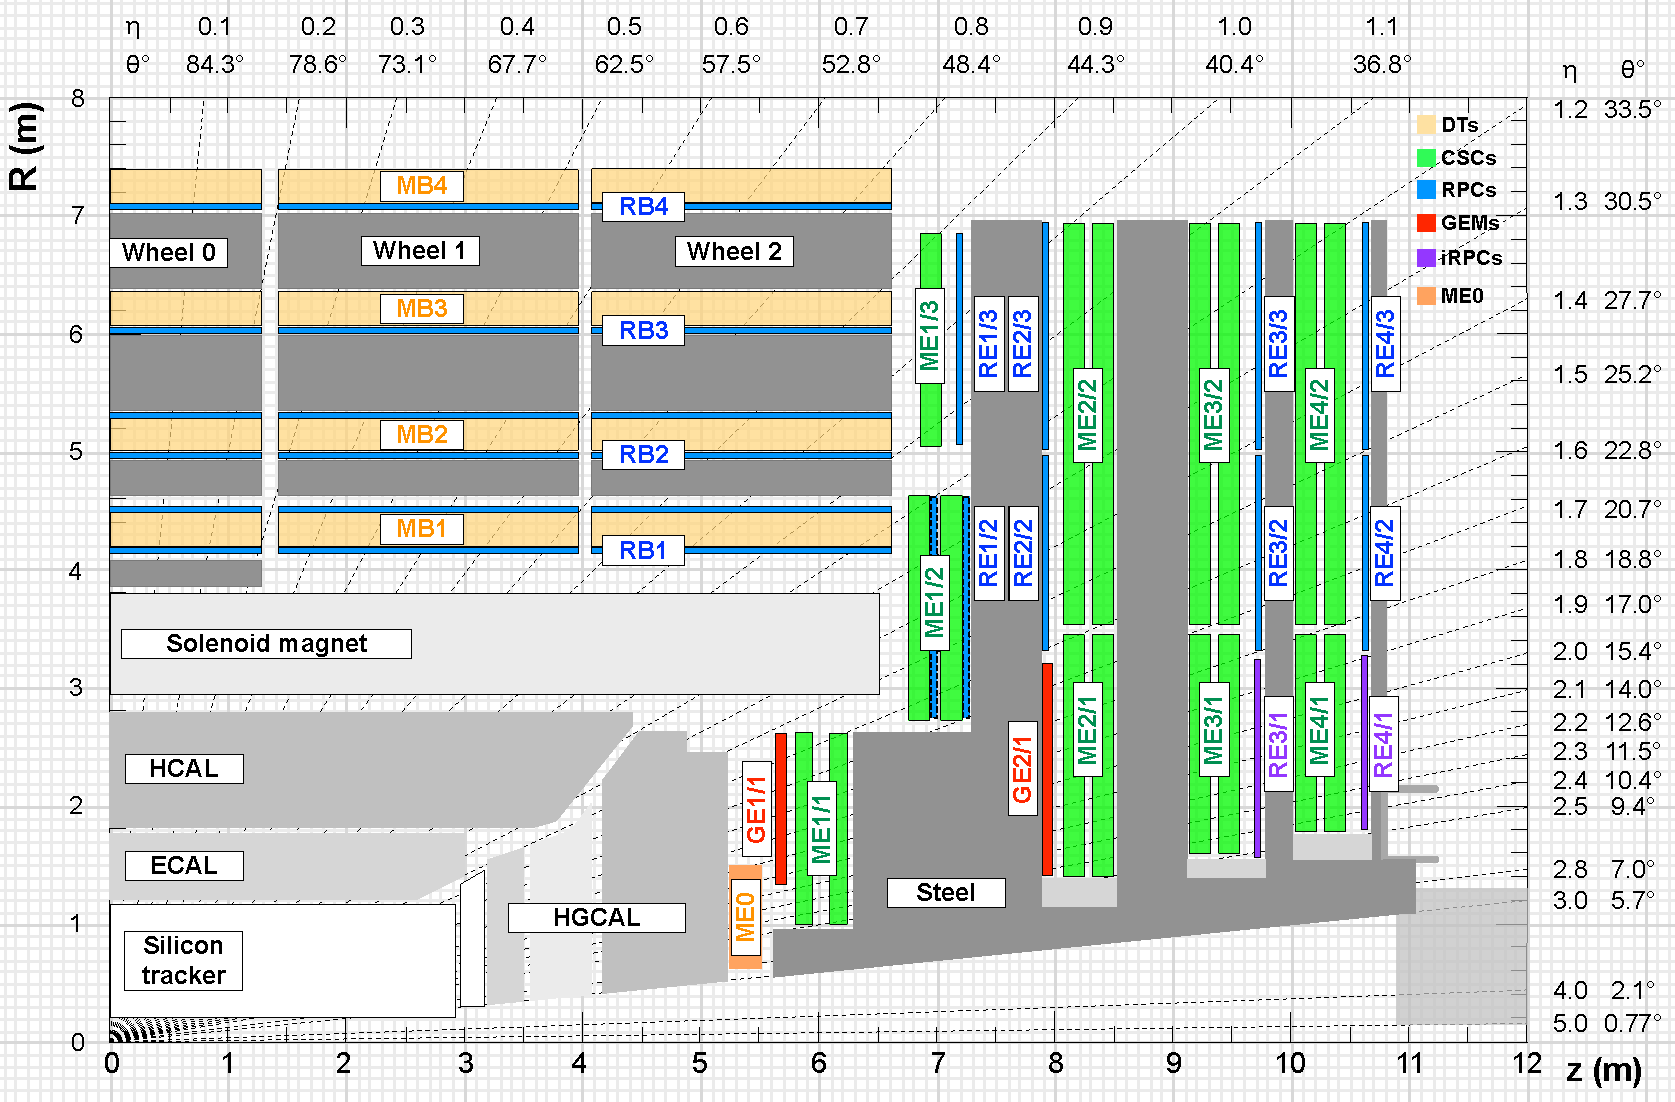
\includegraphics[width=0.9\textwidth]{Figures/Apparatus/cmsphase2upgrade.pdf}
\caption[The Phase-2 CMS muon system]{The Phase-2 CMS muon system~\cite{cmsphase2muons}.}
\label{fig:cmsp2upgrade}
\end{figure}

The Phase-2 L1 system will have a new and flexible architecture (presented in Figure~\ref{fig:cmsl1triggerarchphase2}) to adapt to the HL-LHC data-taking challenges.  The L1 maximum output rate and latency will be increased to 750 kHz and to 12.5 $\mu$s, respectively. Furthermore, these new capabilities will allow for the introduction of a new correlator layer, which will combine inputs from the various trigger systems (muon detectors, calorimeters, tracking detectors) to perform a particle-flow like reconstruction of the event at the hardware trigger level. The L1 system will continue to use state-of-the-art FPGAs equipped with 28 Gb/s transceivers and high-speed optical links, following the successful performance of these technologies during Run-2~\cite{cmsphase1per}.

\begin{figure}[ht!]
\centering
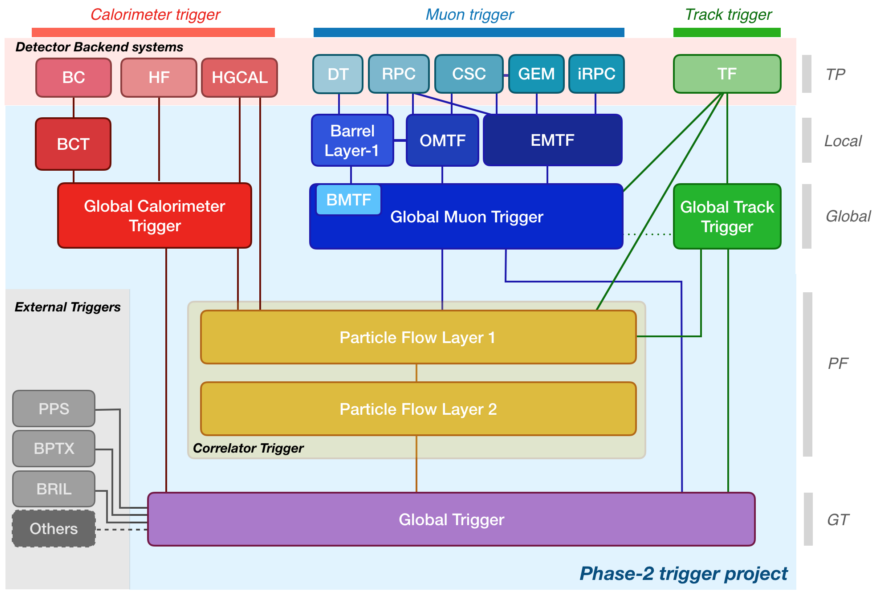
\includegraphics[width=0.9\textwidth]{Figures/Apparatus/cmsl1triggerarchp2.png}
\caption[The Phase-2 Upgrade of the CMS Level-1 trigger architecture]{The Phase-2 Upgrade of the CMS Level-1 trigger architecture~\cite{cmsphase2l1tdr}.}
\label{fig:cmsl1triggerarchphase2}
\end{figure}